\section{Внутренняя геометрия поверхностей}

\subsection{Ковариантное дифференцирование, параллельный перенос}

Пусть $\vec{\gamma}\colon I \to \M$ --- гладкая кривая на поверхности $\M$. Мы будем считать, что она задана в локальных координатах в виде $u^1 = u^1(t)$, $u^2 = u^2(t)$. Пусть для каждого $t \in I$ в касательной плоскости $\T_{\vec{\gamma}(t)}\M$ выбран вектор $\vec{v}(t)$, гладко зависящий от параметра $t$. В этом случае мы будем говорить, что задано \textit{векторное поле вдоль кривой $\vec{\gamma}$}.

Мы хотим построить анализ на поверхности, который будет опираться только на её внутреннюю геометрию. В частности, мы хотим научиться дифференцировать векторные поля вдоль кривых. Обычное дифференцирование нам не подойдёт, ведь поскольку касательные плоскости в разных точках поверхности могут быть различными, производная $\dot{\vec{v}}(t)$, вообще говоря, не задаёт векторного поля к поверхности. Поэтому на неё нельзя смотреть с точки зрения внутренней геометрии поверхности. Рассмотрим вместо этого векторное поля, получающееся проецированием $\dot{\vec{v}}$ на касательное пространство.

\begin{definition}
	\textit{Ковариантной производной} векторного поля $\vec{v}$ вдоль кривой $\vec{\gamma}$ называется векторное поле вдоль этой кривой, обозначаемое через $\nabla_{\dot{\vec{\gamma}}}\vec{v}$ и задаваемое формулой
	\[
		\big(\nabla_{\dot{\vec{\gamma}}}\vec{v}\big)(t) = \proj_{\T_{\vec{\gamma}(t)}\M}\dot{\vec{v}}.
	\]
\end{definition}

Выбранное нами обозначение неспроста сходно с обозначением производной по направлению, смысл этого сходства будет прояснён немного позже. Из определения сразу видны следующие свойства ковариантной производной вдоль пути.

\begin{proposition}
	Ковариантное дифференцирование вдоль фиксированного пути линейно, и подчиняется правилу Ньютона "---Лейбница при умножении на функцию.
\end{proposition}

\begin{definition}
	Говорят, что векторное поле $\vec{v}$ вдоль кривой \textit{ковариантно постоянно} вдоль неё, если его ковариатная производная всюду равна нулю: $\nabla_{\dot{\vec{\gamma}}}\vec{v} \equiv \vec{0}$.
\end{definition}

%Данные выше определения очень естественны и имеют наглядный физический смысл. Чтобы его увидеть, нам нужно ответить на вопрос: какой разумный смысл можно придать словам <<идти прямо>> на поверхности? Хороший взгляд следующий --- положим на поверхность бусинку (которая не будет с неё слетать) и приведём её в движение слабым щелчком без последующего воздействия каких-либо внешних сил. Логично сказать, что тогда бусинка будет <<двигаться прямо>> по поверхности (по направлению, в котором мы её толкнули), при этом на неё действует лишь сила нормальной реакции, всюду перпендикулярная поверхности. Так, мы естественно пришли к точке зрения, что <<идти прямо>> вдоль какого-то направления на поверхности --- это идти так, чтобы вектор нашего ускорения был перпендикулярен этому направлению.

Обобщим данное выше определение ковариантной производной. Пусть теперь векторное поле $\vec{v}$ задано на всей поверхности $\M$, а не только вдоль некоторой кривой. Пусть также $\vec{w} \in \T_{\vec{x}}\M$ --- произвольный касательный вектор к поверхности в точке $\vec{x} \in \M$. Возьмём произвольную гладко параметризованную кривую $\vec{\gamma}(t) = \vec{r}(u^1(t), u^2(t))$ на $\M$, выходящую из точки $\vec{x}$ с вектором скорости $\vec{w}$: $\vec{\gamma}(0) = \vec{x}$, $\dot{\vec{\gamma}}(0) = \vec{v}$ и рассмотрим ограничение поля $\vec{v}$ на эту кривую. Для его ковариантной производной будем иметь
\[
	\big(\nabla_{\dot{\vec{\gamma}}}\vec{v}\big)(t) = \proj_{\T_{\vec{\gamma}(t)}\M}\br{\frac{d}{dt}\vec{v}(\vec{\gamma}(t))} = \proj_{\T_{\vec{\gamma}(t)}\M}\br{\frac{\partial\vec{v}}{\partial u^i}\dot{u}^i}.
\]
При $t = 0$ мы получим
\[
	\big(\nabla_{\dot{\vec{\gamma}}}\vec{v}\big)|_{t = 0} = \proj_{\T_{\vec{x}}\M}(d\vec{v}|_{\vec{x}}(\vec{w})),
\]
то есть вектор, не зависящий от выбора параметризованной кривой. Здесь $d\vec{v}|_{\vec{x}}(\vec{w})$ --- производная векторного поля $\vec{v}$ по направлению вектора $\vec{w}$.

\begin{definition}
	\textit{Ковариантной производной} векторного поля $\vec{v}$ на поверхности $\M$ по направлению вектора $\vec{w} \in \T_{\vec{x}}\M$ в точке $\vec{x}$ называется вектор
	\[
		\big(\nabla_{\vec{w}}\vec{v}\big)(\vec{x}) = \proj_{\T_{\vec{x}}\M}(d\vec{v}|_{\vec{x}}(\vec{w})).
	\]
	\textit{Частными ковариантными производными} $\nabla_i\vec{v}$ назовём ковариантные производные вдоль базисных векторов $\vec{r}_i$ касательной плоскости.
\end{definition}

В этом определении мы взяли производную векторного поля $\vec{v}$ по направлению вектора $\vec{w} \in \T_{\vec{x}}\M$ и спроецировали её на касательную плоскость $\T_{\vec{x}}\M$. Проекция --- линейная операция, а потому для любого вектора $\vec{w} = W^i\vec{r}_i$ выполнено
\[
	\nabla_{\vec{w}}\vec{v} = W^i\nabla_i\vec{v},
\]
так что ковариантная производная по направлению любого вектора однозначно определяется частными ковариантными производными, поэтому полезно вывести общие формулы для последних. Сначала найдём обычные частные производные векторного поля $\vec{v}$:
\begin{equation} \label{eq:PartialVectorField}
	\partial_i\vec{v} = \frac{\partial V^k}{\partial u^i}\vec{r}_k + V^j\vec{r}_{ij} \stackrel{\eqref{eq:DerivativeGauss}}{=\joinrel=} \frac{\partial V^k}{\partial u^i}\vec{r}_k + V^j(\Gamma_{ij}^k\vec{r}_k + b_{ij}\vec{n}).
\end{equation}

Из определения, $\big(\nabla_i\vec{v}\big)(\vec{x}) = \proj_{\T_{\vec{x}}\M}\partial_i\vec{v}$. Спроектировать на касательное пространство частные производные \eqref{eq:PartialVectorField} --- значит убрать у них слагаемые с $\vec{n}$. Получаем:
\[
	\nabla_i\vec{v} = \br{\frac{\partial V^k}{\partial u^i} + \Gamma_{ij}^kV^j}\vec{r}_k.
\]
Часто эту формулу записывают так:
\begin{equation} \label{eq:CovariantVectorField}
	\big(\nabla_i\vec{v}\big)^k = \frac{\partial V^k}{\partial u^i} + \Gamma_{ij}^kV^j
\end{equation}

Выбор коэффициентов $\Gamma_{ij}^k$ так, чтобы выражение \eqref{eq:CovariantVectorField} не зависело от выбора системы координат, называется \textit{связностью} (на многообразии). Определяя $\Gamma_{ij}^k$ как символы Кристоффеля, то есть по тождествам \eqref{eq:ChristoffelIdentity}, мы получаем \textit{симметричную риманову связность}. В этом курсе мы будем сталкиваться только с ней.

Итак, общая формула ковариантной производной по направлению имеет вид
\begin{equation} \label{eq:CovariantFormula}
	\big(\nabla_{\vec{w}}\vec{v}\big)^k = \big(W^i\nabla_i\vec{v}\big)^k = W^i\frac{\partial V^k}{\partial u^i} + \Gamma_{ij}^kW^iV^j.
\end{equation}

%Отметим глубинный смысл формулы, полученной нами при решении задачи \ref{problem:ChristoffelNotTensor}. Дело в том, что нетензорный характер преобразования символов Кристоффеля компенсирует <<нетензорность>> частной производной. (Ведь ковариантная производная уже обязана меняться, как тензор!) В частности, с помощью этого наблюдения можно более простым путём прийти к формуле преобразования символов Кристоффеля, выведенной нами ранее лобовыми вычислениями.

\begin{proposition} \label{proposition:TranslationProperties}
	Для любых векторных полей $\vec{v}$, $\vec{v}_1$, $\vec{v}_2$ и векторов $\vec{w}$, $\vec{w}_1$, $\vec{w}_2$ в фиксированной точке $\vec{x}$ поверхности, функции $f$ на $\M$, а также чисел $\lambda_1$, $\lambda_2$ выполнено следующее:
	\begin{gather*}
		\nabla_{\vec{w}}(\vec{v}_1 + \vec{v}_2) = \nabla_{\vec{w}}\vec{v}_1 + \nabla_{\vec{w}}\vec{v}_2,\\
		\nabla_{\vec{w}}(f\vec{v}) = (\nabla_{\vec{w}}f)\vec{v} + f(\nabla_{\vec{w}}\vec{v}),\\
		\nabla_{\lambda_1\vec{w}_1 + \lambda_2\vec{w}_2}\vec{v} = \lambda_1\nabla_{\vec{w}_1}\vec{v} + \lambda_2\nabla_{\vec{w}_2}\vec{v},\\
		\nabla_{\vec{w}}\langle\vec{v}_1, \vec{v}_2\rangle = \langle\nabla_{\vec{w}}\vec{v}_1, \vec{v}_2\rangle + \langle\vec{v}_1, \nabla_{\vec{w}}\vec{v}_2\rangle,
	\end{gather*}
	где $(\nabla_{\vec{w}}f)(\vec{x}) \vcentcolon = df|_{\vec{x}}(\vec{w})$ --- производная функции $f$ по направлению вектора $\vec{w}$.
\end{proposition}

\begin{proof}
	Первые три равенства проверяются непосредственно. Для доказательства последнего нам пригодится тождество \eqref{eq:AlmostCristoffelIdentity}:
	\begin{multline*}
		\nabla_{\vec{w}}\langle\vec{v}_1, \vec{v}_2\rangle = W^k\frac{\partial}{\partial u^k}(V_1^iV_2^jg_{ij}) = W^k\br{\frac{\partial V_1^i}{\partial u^k}V_2^jg_{ij} + V_1^i\frac{\partial V_2^j}{\partial u^k}g_{ij} + V_1^iV_2^j\frac{\partial g_{ij}}{\partial u^k}} =\\ = W^k\br{\frac{\partial V_1^i}{\partial u^k}V_2^jg_{ij} + V_1^i\frac{\partial V_2^j}{\partial u^k}g_{ij} + V_1^iV_2^j(g_{js}\Gamma_{ik}^s + g_{is}\Gamma_{jk}^s)} =\\ = \underbrace{W^k\br{\frac{\partial V_1^i}{\partial u^k} + \Gamma_{sk}^iV_1^s}}_{\nabla_{\vec{w}}\vec{v}_1}V_2^jg_{ij} + \underbrace{W^k\br{\frac{\partial V_2^j}{\partial u^k} + \Gamma_{sk}^jV_2^s}}_{\nabla_{\vec{w}}\vec{v}_2}V_1^ig_{ij} = \langle\nabla_{\vec{w}}\vec{v}_1, \vec{v}_2\rangle + \langle\vec{v}_1, \nabla_{\vec{w}}\vec{v}_2\rangle.
	\end{multline*}
	В предпоследнем равенстве мы переобозначили несколько индексов. Выкладка выглядит не совсем прозрачной, но в ней нетрудно разобраться.
\end{proof}

Вернёмся к ковариатной производной вдоль кривой $\vec{\gamma}(t) = \vec{r}(u^1(t), u^2(t))$. При подстановке $\vec{w} = \dot{\vec{\gamma}}$ в формулы \eqref{eq:CovariantFormula} получим
\[
	\big(\nabla_{\dot{\vec{\gamma}}}\vec{v}\big)^k = \big(\dot{\gamma}^i\nabla_i\vec{v}\big)^k = \dot{u}^i\frac{\partial V^k}{\partial u^i} + \dot{u}^i\Gamma_{ij}^kV^j = \frac{dV^k}{dt} + \Gamma_{ij}^k\dot{u}^iV^j.
\]

\begin{theorem}
	Для любого гладкого пути $\vec{\gamma}\colon [0; 1] \to \M$ на поверхности $\M$ и любого касательного вектора $\vec{\xi} \in \T_{\vec{\gamma}(0)}\M$ существует и единственно векторное поле $\vec{v}(t)$, ковариантно постоянное вдоль этого пути и такое, что $\vec{v}(0) = \vec{\xi}$.
\end{theorem}

\begin{proof}
	Утверждение теоремы следует из того, что условие ковариантной постоянности поля вдоль кривой равносильно следующей системе линейных дифференциальных уравнений на координаты $(V^1, V^2)$ вектора $\vec{v}$ в базисе $(\vec{r}_1, \vec{r}_2)$:
	\[
		\dot{V}^k(t) = \Gamma_{ij}^k(u^1(t), u^2(t))V^j(t)\dot{u}^k(t).
	\]
\end{proof}

Подчеркнём, что линейность этих уравнений даёт возможность продолжить решение при всех $t$. Таким образом, для любой кривой по начальному касательному вектору в некоторой её точке мы можем однозначно построить в каждой точке этой кривой касательный вектор таким образом, чтобы векторное поле, образованное всеми этими векторами, было ковариантно постоянным вдоль нашей кривой.

\begin{definition}
	\textit{Параллельным переносом} вектора $\vec{\xi}$ вдоль кривой $\vec{\gamma}(t)$ называется построение векторного поля $\vec{v}(t)$, для которого $\vec{v}(0) = \vec{\xi}$ и $\nabla_{\dot{\vec{\gamma}}}\vec{v} \equiv \vec{0}$:
	\begin{equation} \label{eq:ParallelTranslation}
		\frac{dV^k}{dt} + \Gamma_{ij}^k\dot{\gamma}^iV^j = 0.
	\end{equation}
	Уравнения \eqref{eq:ParallelTranslation} при этом называются \textit{уравнениями параллельного переноса}.
\end{definition}

\begin{lemma}
	Параллельный перенос сохраняет скалярное произведение. В частности, при параллельном переносе сохраняются длины векторов и углы между ними.
\end{lemma}

\begin{proof}
	Достаточно проверить, что при параллельном переносе сохраняются длины векторов (так как билинейная форма однозначно восстанавливается по соответствующей ей квадратичной форме). А это следует из того, что для векторного поля $\vec{v}$, ковариантно постоянного вдоль некоторого пути на поверхности, выполнено $\vec{v} \perp \dot{\vec{v}}$ сразу из определения ковариантной производной.
\end{proof}

Таким образом, при параллельном переносе вдоль любой кривой касательные вектора остаются неподвижными друг относительно друга. А значит, во время параллельного переноса касательная плоскость может лишь целиком поворачиваться в пространстве. Возникает естественный вопрос, а обязательно ли при параллельном переносе по замкнутой траектории касательная плоскость перейдёт в себя?

\begin{problem} \label{problem:SphereTranslation}
	На какой угол повернётся касательный вектор к единичной сфере после параллельного переноса вдоль параллели $\theta = \theta_0$ ($0 \leqslant \theta_0 \leqslant \frac{\pi}{2}$) на угол $2\pi$?
\end{problem}

\begin{firstsolution}
	Напомним, что параметризация $\vec{r}(\theta, \varphi)$ единичной сферы имеет вид
	\[
		x = \sin\theta\cos\varphi,\quad y = \sin\theta\sin\varphi,\quad z = \cos\theta,
	\]
	где $0 \leqslant \theta \leqslant \pi$, $0 \leqslant \varphi < 2\pi$. Отсюда можем легко найти первую квадратичную форму сферы:
	\[
		\G =
		\begin{pmatrix}
			1 & 0\\
			0 & \sin^2\theta
		\end{pmatrix}.
	\]

	Глобально мы хотим написать уравнение \eqref{eq:ParallelTranslation} параллельного переноса вдоль замкнутой кривой $\theta = \theta_0$ и решить его. Для этого нам нужно сначала найти символы Кристоффеля, воспользовавшись для этого тождествами Кристоффеля. Сначала хорошо бы явно выписать обратную матрицу метрики:
	\[
		\G^{-1} = \frac{1}{\sin^2\theta}
		\begin{pmatrix}
			\sin^2\theta & 0\\
			0 & 1
		\end{pmatrix}.
	\]

	Отметим два полезных факта: во-первых, метрика $\G$ зависит только от значения параметра $\theta$, а во-вторых, матрицы $\G$ и $\G^{-1}$ диагональные. Это существенно сокращает вычиления. Получаем, что единственными ненулевыми символами Кристоффеля оказываются
	\[
		\Gamma_{22}^1 = -\sin\theta\cos\theta,\quad \Gamma_{12}^2 = \Gamma_{21}^2 = \ctg\theta.
	\]

	Параллель $\theta = \theta_0$ в нашей параметризации параметризуется следующим образом: $\theta(t) \hm= \theta_0$, $\varphi(t) = t$, $0 \leqslant t < 2\pi$. Тогда $\dot{\theta} = 0$, $\dot{\varphi} = 1$. Уравнения параллельного переноса \eqref{eq:ParallelTranslation}
	\[
		\frac{dV^k}{dt} + \Gamma_{ij}^k\dot{\gamma}^iV^j = 0
	\]
	в нашем случае имеют вид
	\[
		\begin{cases}
			\begin{aligned}
				&\frac{dV^1}{dt} + \Gamma_{22}^1\dot{\varphi}V^2 = 0,\\
				&\frac{dV^2}{dt} + \underbrace{\Gamma_{12}^2\dot{\theta}V^2}_{0} + \Gamma_{21}^2\dot{\varphi}V^1 = 0
			\end{aligned}
		\end{cases} \Rightarrow
		\begin{cases}
			\begin{aligned}
				&\frac{dV^1}{dt} - \sin\theta_0\cos\theta_0V^2 = 0,\\
				&\frac{dV^2}{dt} + \ctg\theta_0V^1 = 0.
			\end{aligned}
		\end{cases}
	\]

	Это однородная линейная система обыкновенных дифференциальных уравнений на компоненты $(V^1, V^2)$ поля. Можно продемонстрировать мастерство и решить её стандартными методами, изученными в рамках соответствующего курса. Но мы схитрим --- продифференцируем первое уравнение
	\[
		\frac{dV^2}{dt} = \frac{1}{\sin\theta_0\cos\theta_0}\frac{d^2V^1}{dt^2}
	\]
	и поставим во второе:
	\[
		\frac{1}{\cancel{\sin\theta_0}\cos\theta_0}\frac{d^2V^1}{dt^2} + \frac{\cos\theta_0}{\cancel{\sin\theta_0}}V^1 = 0.
	\]
	Получаем уравнение малых колебаний:
	\[
		\frac{d^2V^1}{dt^2} + \cos^2\theta_0V^1 = 0.
	\]

	На самом деле, дальше нам дорешивать ничего не нужно. Отсюда мы уже видим, что при таком параллельном переносе вектор вращается с амплитудой $\cos\theta_0$. Так что при полном обороте вокруг параллели вектор повернётся на угол $2\pi\cos\theta_0$.
\end{firstsolution}

Из последней задачи видно, что при параллельном переносе по замкнутой траектории вектор может не перейти в себя, но повернуться на некоторый угол. Этот эффект вызван кривизной поверхности, по которой осуществляется перенос.

Отметим, что по определению ковариантная производная векторного поля $\vec{v}$ вдоль кривой $\vec{\gamma}$ зависит только от векторного поля, кривой и положения касательной плоскости в точках кривой, так что очевидно следующее предложение.

\begin{proposition}
	Пусть поверхности $\M_1$ и $\M_2$ касаются по кривой $\vec{\gamma}$. Тогда векторное поле, ковариантно постоянное вдоль $\vec{\gamma}$ по отношению к $\M_1$ является таковым и по отношению к $\M_2$.
\end{proposition}

Отсюда немедленно извлекаем, что если кривая лежит в пересечении двух поверхностей, то результат параллельного переноса любого вектора вдоль этой кривой не зависит от того, по какой именно поверхности осуществлялся перенос.

Это наблюдение часто помогает упрощать рассуждения в задачах, где фигурирует параллельный перенос. Действительно, ведь можно заменить данную нам поверхность на ту, в которой параллельный перенос выглядит проще. Пользуясь этим трюком, приведём ещё одно решение задачи \ref{problem:SphereTranslation}.

\begin{secondsolution}
	Рассмотрим конус, пересекающийся с единичной сферой по параллели $\theta = \theta_0$. (Здесь есть два особых случая $\theta_0 = 0$ и $\theta_0 = \frac{\pi}{2}$, в которых мы получаем плоскость и цилиндр соответственно, но для дальнейших рассуждений нам это ничем не помешает.) Будем вместо сферы выполнять параллельный перенос по этому конусу, результат от этого не зависит.

	Рассмотрим развёртку этого конуса, то есть отобразим его локально изометрично на плоскость. (Для этого конус необходимо <<разрезать>>, но нас это тоже не волнует.) Так как уравнение параллельного переноса и значение угла между векторами зависят только от метрики, то можно осуществить параллельный перенос данного вектора по развёртке, результат также не поменяется. А в развёртке мы получаем параллельный перенос вектора по дуге окружности (в которую развернётся наша параллель). В начале этот вектор касается окружности, а так как в плоскости параллельный перенос устроен тривиально, он и в конце будет её касаться.

	Легко находим угол между осью и образующей нашего конуса равен $\frac{\pi}{2} - \theta_0$, а значит, угол при вершине конуса в развёртке будет равен
	\[
		2\pi\sin\br{\frac{\pi}{2} - \theta_0} = 2\pi\cos\theta_0.
	\]

	Легко видеть, что это и есть угол, на который повернётся наш вектор при параллельном переносе вдоль дуги окружности.
\end{secondsolution}

\subsection{Геодезические линии}

\begin{definition}
	Кривая $\vec{\gamma}(t)$, параметризация которой пропорциональна натуральной, называется \textit{геодезической линией}, если $\nabla_{\dot{\vec{\gamma}}}\dot{\vec{\gamma}} \equiv \vec{0}$:
	\begin{equation} \label{eq:Geodesic}
		\ddot{\gamma}^k + \Gamma_{ij}^k\dot{\gamma}^i\dot\gamma^j = 0.
	\end{equation}
	Уравнения \eqref{eq:Geodesic} называют \textit{уравнениями геодезической}.
\end{definition}

Далее мы будем называть параметр, пропорциональный натуральному, \textit{аффинным натуральным} параметром. (Ведь этот параметр получается из натурального аффинным преобразованием.)

Геодезические --- это те кривые, которые будет вырисовывать бусинка, двигаясь по поверхности без воздействия внешних сил. Уравнения \eqref{eq:Geodesic} --- это дифференциальные уравнения уже второго порядка, а потому начальными условиями для него служат точка $\vec{\gamma}(0)$ и вектор скорости $\dot{\vec{\gamma}}(0)$ --- куда положить бусинку и в какую сторону её толкнуть. Таким образом, геодезические линии на искривлённой поверхности служат аналогами прямых на плоскости. В дальнейшем мы будем развивать эту интуицию.

Итак, мы знаем, что для каждой внутренней точки $\vec{x}$ поверхности $\M$ и ненулевого касательного вектора $\vec{v} \in \T_{\vec{x}}\M$ существует ровно одна геодезическая дуга достаточно малой длины, начинающаяся в точке $\vec{x}$ и выходящая из неё в направлении $\vec{v}$. Рассмотрим вопрос о продолжаемости геодезических.

\begin{theorem}
	Пусть $\vec{x}$ --- внутренняя точка поверхности $\M$, $\vec{v} \in \T_{\vec{x}}\M$ --- ненулевой касательный вектор. Тогда на $\M$ существует геодезическая с аффинным натуральным параметром $\vec{\gamma}(t)$, выходящая при $t = 0$ из точки $\vec{x}$ в направлении вектора $\vec{v}$ и продолжаемая либо бесконечно, либо до края $\partial\M$ данной поверхности.
\end{theorem}

\begin{proof}
	Рассмотрим сначала параметризованный простой кусок $\mathcal{N}$ данной поверхности, для которого данная точка $\vec{x}$ внутренняя. Координаты в $\mathcal{N}$ будем, как обычно, обозначать через $(u^1, u^2)$. Координаты точки $\vec{x}$ обозначим через $(u_0^1, u_0^2)$. Построение начального куска искомой геодезической сводится к решению уравнения \eqref{eq:Geodesic} с начальными условиями в точке $\vec{x}$ и начальным вектором скорости $\vec{v} / |\vec{v}|$ (начальный вектор для удобства нормируем). Согласно теореме \ref{theorem:ContinuityDifferential} о продолжении решений обыкновенного дифференциального уравнения, этот начальный кусок можно продолжить до границы любого наперёд заданного компакта в фазовом пространстве.

	Напомним, что координатами в фазовом пространстве служат $(u^1, u^2, \dot{u}^1, \dot{u}^2)$. При попытке продолжения решения до границы компакта мы можем <<упереться>> в его границу по координатам $u^1$ или $u^2$ (что будет соответствовать тому, что мы дошли до края $\partial\mathcal{N}$ нашего куска), либо же по координатам $\dot{u}^1$ или $\dot{u}^2$. Докажем, что мы можем выбрать такой компакт в фазовом пространстве, что будет реализовываться именно первый случай.

	Ключевую роль здесь играет тот факт, что в силу уравнений \eqref{eq:Geodesic} длина вектора скорости сохраняется: $g_{ij}\dot{u}^i\dot{u}^j = 1$.

	\begin{lemma}
		Существует $\eps > 0$ такое, что во всех точках $(u^1, u^2)$ куска поверхности $\mathcal{N}$ для любого ненулевого касательного вектора $\vec{w} = W^i\vec{r}_i$ выполнено неравенство
		\[
			g_{ij}W^iW^j > \eps\big((W^1)^2 + (W^2)^2\big).
		\]
	\end{lemma}

	\begin{proof}
		Пусть $\lambda(u^1, u^2)$ --- меньшее из собственых значений матрицы $(g_{ij})$. Если $\eps < \lambda$, то матрица $\G - \eps E$ положительно определена. На компактном куске $\mathcal{N}$ (напомним, что простой кусок поверхности гомеоморфен диску) непрерывная функция $\lambda$ достигает минимума $\lambda_{\min} > 0$. Любая константа на интервале $0 < \eps < \lambda_{\min}$ удовлетворяет условию во всех точках куска $\mathcal{N}$.
	\end{proof}

	Из только что доказанной леммы следует, что вдоль решения $(u^1(t), u^2(t))$ выполнено неравенство
	\begin{equation} \label{eq:EpsInequality}
		(\dot{u}^1)^2 + (\dot{u}^2)^2 < 1 / \eps
	\end{equation}
	для некоторого $\eps > 0$. Вооружившись такой константой $\eps$, рассмотрим компакт в фазовом пространстве, задаваемый некоторыми неравенствами на $u^1$, $u^2$ (чтобы не <<вылезти>> за границы куска $\mathcal{N}$) и неравенством $(\dot{u}^1)^2 + (\dot{u}^2)^2 \leqslant 1 / \eps$. Дойти до границы по $\dot{u}^1$ или $\dot{u}^2$ нам мешает неравенство \eqref{eq:EpsInequality}, так что решение либо продолжается неограниченно внутри этого компакта (внутри куска $\mathcal{N}$), либо <<упирается>> в границу по $u^1$ или $u^2$ (в край $\partial\mathcal{N}$).

	Забудем теперь о фиксированном куске $\mathcal{N}$. Пусть $t_{\max}$ --- это супремум тех $t$, для которых возможно продолжить геодезическую $\vec{\gamma}(t)$. Если $t_{\max} = +\infty$, то теорема доказана. Иначе, существует предел
	\[
		\lim_{t \to t_{\max}-}\vec{\gamma}(t) = \vcentcolon \vec{x}_1,
	\]
	поскольку вектор скорости $\dot{\vec{\gamma}}(t)$ единичный для всех $t < t_{\max}$. Значит, кривая $\vec{\gamma}(t)$ определена и при $t = t_{\max}$. Если точка $\vec{x}_1$ внутренняя для поверхности $\M$, то можно применить рассуждение выше и показать, что решение продолжается дальше $t_{\max}$, что противоречит выбору последнего. Следовательно, $\vec{x}_1 \in \partial\M$, и мы продолжили решение до края поверхности.
\end{proof}

% TODO: Нормально написать про теорему Хопфа-Ринова

\begin{problem}
	Найти геодезические на геликоиде.
\end{problem}

\begin{solution}
	Напомним, что параметризация $\vec{r}(u, v)$ геликоида имеет вид
	\[
		x = u\sin v,\quad y = u\cos v,\quad z = v,
	\]
	где $u, v \in \R$. Находим метрику:
	\[
		\G =
		\begin{pmatrix}
			1 & 0\\
			0 & u^2 + 1
		\end{pmatrix}.
	\]
	Затем находим символы Кристоффеля. Аналогично прошлой задаче получим, что единственные ненулевые символы есть
	\[
		\Gamma_{22}^1 = -u,\quad \Gamma_{12}^2 = \frac{u}{u^2 + 1}.
	\]
	Теперь хотим написать уравнения геодезических \eqref{eq:Geodesic}
	\[
		\ddot{\gamma}^k + \Gamma_{ij}^k\dot{\gamma}^i\dot{\gamma}^j = 0
	\]
	и решить их. В нашем случае уравнения имеют следующий вид:
	\[
		\begin{cases}
			\ddot{u} + \Gamma_{22}^1\dot{v}^2 = 0,\\
			\ddot{v} + 2\Gamma_{12}^2\dot{u}\dot{v} = 0
		\end{cases} \Rightarrow
		\begin{cases}
			\begin{aligned}
				&\ddot{u} - u\dot{v}^2 = 0,\\
				&\ddot{v} + \frac{2u\dot{u}}{u^2 + 1}\dot{v} = 0.
			\end{aligned}
		\end{cases}
	\]

	Заметим, что можно домножить второе уравнение на $u^2 + 1$, получив в левой части полный дифференциал. Тогда получаем следующие уравнения:
	\[
		\begin{cases}
			\begin{aligned}
				&\ddot{u} - u\dot{v}^2 = 0,\\
				&\frac{d}{dt}\big((u^2 + 1)\dot{v}\big) = 0.
			\end{aligned}
		\end{cases}
	\]

	Получаем, что $(u^2 + 1)\dot{v} = C_1$ ($C_1 \in \R$). Отсюда выражаем $\dot{v} = C_1 / (u^2 + 1)$ и подставляем в первое уравнение:
	\[
		\ddot{u} - \frac{C_1^2u}{(u^2 + 1)^2} = 0.
	\]

	Чтобы решить это уравнение, необходимо вспомнить трюк из задачника Филиппова: рассмотрим $\dot{u}$ как функцию $P(u)$ от $u$. В таких обозначениях будем иметь
	\[
		\ddot{u} = \frac{d}{dt}(\dot{u}) = \frac{d}{dt}(P(u)) = \dot{u}P^\prime = PP^\prime.
	\]
	(Здесь штрихом обозначена производная по $u$.) Подставляем:
	\begin{gather*}
		PP^\prime - \frac{C_1^2u}{(u^2 + 1)^2} = 0,\quad PdP = \frac{C_1^2u}{(u^2 + 1)^2}du,\\
		\int PdP = C_1^2\int\frac{udu}{(u^2 + 1)^2}.
	\end{gather*}
	Первообразная в левой части с точностью до константы есть $\frac{P^2}{2}$. Интеграл в правой части легко считается:
	\[
		\int\frac{udu}{(u^2 + 1)^2} = \frac{1}{2}\int\frac{d(u^2 + 1)}{(u^2 + 1)^2} = -\frac{1}{2(u^2 + 1)} + C.
	\]
	Итого получаем
	\[
		P^2 = -\frac{C_1^2}{(u^2 + 1)} + C_2.
	\]

	Явно это дифференциальное уравнение уже не решается. Но мы получили возможность в приемлемом виде выразить ответ:
	\begin{gather*}
		du = \pm\sqrt{-\frac{C_1^2}{(u^2 + 1)} + C_2}\,dt,\\
		\frac{dv}{du} = \pm\frac{C_1}{(u^2 + 1)\sqrt{-\frac{C_1^2}{(u^2 + 1)} + C_2}} = \pm\frac{C_1}{\sqrt{C_2(u^2 + 1)^2 - C_1^2(u^2 + 1)}}.
	\end{gather*}
\end{solution}

\begin{problem} \label{eq:GeodesicSphere}
	Доказать, что геодезические на сфере суть большие круги.
\end{problem}

\begin{proof}
	Можно решать эту задачу так же, как мы делали это для геликоида --- считать символы Кристоффеля, выписывать уравнения геодезических, решать их и сверять ответ. Но мы так делать не будем\footnotemark.

	\footnotetext{<<При виде дифференциального уравнение сначала подумайте, как бы его не решать>>, --- А.\,В. Пенской.}

	Сначала проверим, что большие круги действительно являются геодезическими. Пусть кривая $\vec{\gamma}$ в натуральной параметризации задаёт большой круг. Тогда очевидно, что $\ddot{\vec{\gamma}}$ задаёт нормаль к сфере, а это значит, что $\nabla_{\dot{\vec{\gamma}}}\dot{\vec{\gamma}} \equiv \vec{0}$.

	Ясно, что для каждой точки и каждого направления существует большой круг, проходящей через данную точку в этом направлении, и он является геодезической. Но по теореме о существовании и единственности для решений обыкновенных дифференциальных уравнений больше никаких геодезических быть не может, ведь мы умеем строить решение уравнения \eqref{eq:Geodesic} для каждого начального условия.
\end{proof}

Трюк, которым мы воспользовались в решении последней задачи, очень важен с практической точки зрения. Мы ещё будем им пользоваться для нахождения геодезических на плоскости Лобачевского.

Можем сделать ещё одно наблюдение, упрощающее поиск геодезических. Пусть мы доказали, что некоторая кривая $\vec{\gamma}$ на поверхности $\M$ является геодезической (это можно сделать, просто подставив её в уравнение). Тогда рассмотрим любую изометрию $\vec{f}\colon \M \to \M$. Так как изометрия сохраняет метрику, то и кривая $\vec{f}(\vec{\gamma})$ тоже будет геодезической. (Ведь уравнение геодезических \eqref{eq:Geodesic} целиком определяется метрикой.)

Приведём здесь ещё два полезных наблюдения, часто пригождающихся в решении задач, связанных с геодезическими и параллельным переносом.

\begin{proposition}
	Если прямая целиком лежит в поверхности, то она является геодезической на этой поверхности.
\end{proposition}

\begin{proof}
	Пусть $\vec{\gamma}$ --- натуральный параметризация данной прямой. Тогда
	\[
		(\nabla_{\dot{\vec{\gamma}}}\dot{\vec{\gamma}})(\vec{x}) = \proj_{\T_{\vec{x}}\M}\underbrace{\frac{d}{dt}\dot{\vec{\gamma}}}_{\ddot{\vec{\gamma}} = \vec{0}} = \vec{0}.
	\]
	Таким образом, $\vec{\gamma}$ --- геодезическая по определению.
\end{proof}

\begin{proposition}
	Если $\vec{\gamma}$ --- геодезическая, то при параллельном переносе вектора $\vec{\xi}$ вдоль $\vec{\gamma}$ угол между ним и $\vec{\gamma}$ не меняется.
\end{proposition}

Как мы помним, при параллельном переносе касательная плоскость может целиком поворачиваться на некоторый угол. Последнее предложение говорит нам о том, что при параллельном переносе вдоль геодезической касательная плоскость остаётся неподвижной.

\begin{proof}
	Параллельный перенос вектора $\vec{\xi}$ вдоль $\vec{\gamma}$ --- это процесс построения ковариантно постоянного вдоль $\dot{\vec{\gamma}}$ векторного поля $\vec{v}$ такого, что $\vec{v}(0) = \vec{\xi}$. Из определения геодезической $\nabla_{\dot{\vec{\gamma}}}\dot{\vec{\gamma}} = \vec{0}$, поэтому при параллельном переносе вектор скорости геодезической переходит в себя. При этом параллельный перенос сохраняет углы, поэтому для каждого $t$ имеем $\angle(\vec{v}(t), \dot{\vec{\gamma}}) = \angle(\vec{\xi}, \dot{\vec{\gamma}})$, что и требовалось.
\end{proof}

Для кривых в $\R^n$ мы определяли кривизну --- величину, выражающую степень отличия кривой от прямой. Поэтому на поверхностях кажется естественным определить величину, выражающую степень отличия кривой от геодезической.

Вектор $\vec{k}_g \vcentcolon = \nabla_{\dot{\vec{\gamma}}}\dot{\vec{\gamma}}$ называется \textit{вектором геодезической кривизны} кривой $\vec{\gamma}$ (здесь на кривой $\vec{\gamma}$ введён натуральный параметр). Геодезической кривизной (по аналогии с плоским случаем) можно было бы назвать длину этого вектора, однако мы поступим иначе. Так же, как и для кривых на плоскости, геодезической кривизне линии на двумерной поверхности имеет смысл приписывать знак, если кривая коориентирована в смысле следующего определения.

\begin{definition}
	\textit{Коориентацией} кусочно-гладкой кривой $\vec{\gamma}$ \textit{на поверхности} $\M$ называется согласованный выбор в каждой её точке гладкости $\vec{x}$ единичного вектора $\vec{n}_g$, касательного к поверхности ортогонального кривой $\vec{\gamma}$ в этой точке. Согласованность означает, что при введении на $\vec{\gamma}$ параметризации, которая регулярна на каждой гладкой дуге, вектор нормали к поверхности, определённый из равенста
	\[
		\vec{n} = \frac{\vec{n}_g \times \vec{v}}{\abs{\vec{n}_g \times \vec{v}}},
	\]
	где $\vec{v}$ --- вектор скорости кривой, непрерывно зависит от точки кривой там, где кривая гладкая и непрерывно продолжается на те точки, где вектор скорости $\vec{v}$ меняется скачком. (В частности, если кривая замкнута, то векторы нормали $\vec{n}$ в начальный и конечный моменты должны быть одинаковы.)
\end{definition}

Заметим, что кривая может иметь коориентацию и на поверхности, на которой нельзя всюду определить единичный вектор нормали $\vec{n}$ так, чтобы он непрерывно зависел от точки поверхности. Например, можно обогнуть гладкой кривой ленту Мёбиуса, вернувшись в ту же точку, но сменив направление вектора нормали. Однако её границу можно коориентировать (например, направив все вектора $\vec{n}_g$ внутрь поверхности).

\begin{figure}[H]
	\centering
	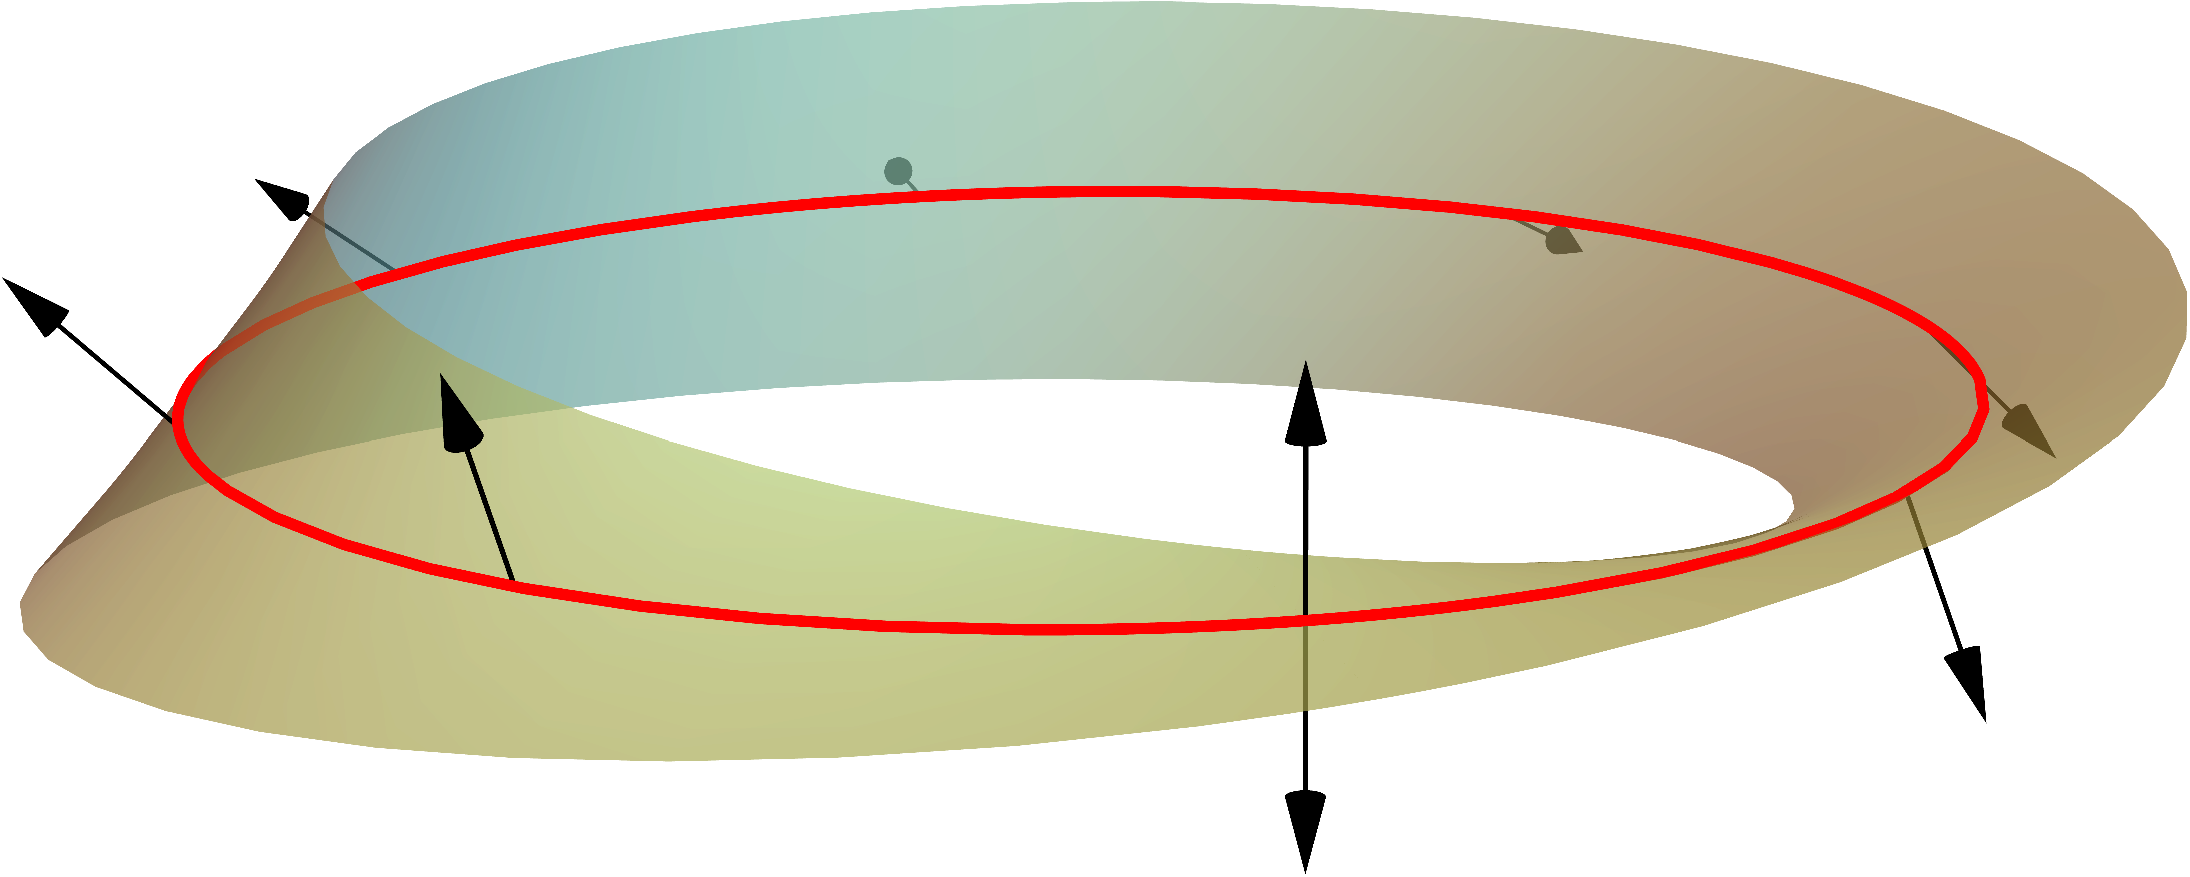
\includegraphics[width=10cm]{./img/MobiusStrip.pdf}
	\caption{Лента Мёбиуса --- пример\\ неориентируемой поверхности}
\end{figure} % TODO: добавить на картинку коориентацию границы?

Отметим также, что на неориентируемой поверхности некоторые замкнутые кривые нельзя коориентировать. Если же это можно сделать, то ровно двумя способами.

Легко видеть, что в каждой точке коориентированной кривой выполнено $\vec{k}_g \parallel \vec{n}_g$, так что можем определить геодезическую кривизну (со знаком) также, как мы это делали для ориентированной кривизны на плоскости.

\begin{definition}
	\textit{Геодезической кривизной} коориентированной кривой на двумерной поверхности называется гладкая функция $k_g\vcentcolon = \langle\vec{k}_g, \vec{n}_g\rangle$.
\end{definition}

В случае, когда $\M$ --- евклидова плоскость, геодезическая кривизна совпадает с ориентированной кривизной плоской кривой. Очевидны также следующие утверждения.

\begin{proposition}
	Кривая $\vec{\gamma}$ является геодезической тогда и только тогда, когда её геодезическая кривизна всюду равна нулю.
\end{proposition}

\begin{proposition}
	При изометрии поверхностей геодезические кривизны всех кривых сохраняются. В частности, геодезические линии переходят в геодезические.
\end{proposition}

Последнее предложение вытекает из того, что геодезическая кривизна, как легко видеть, однозначно определяется метрикой. (Строго говоря, важен ещё выбор коориентации на кривых, ведь иначе утверждение верно лишь с точностью до знака. Но коориентации на двух кривых всегда можно выбрать согласованно.)

Мы видели, что кривизна плоской кривой равна скорости вращения вектора скорости при условии, что длина последнего равна единице. Аналогичное утверждение верно для геодезической кривизны кривой на произвольной поверхности, только теперь вектор скорости вращается не в неподвижной плоскости, а в касательной плоскости к поверхности, которая движется вместе с точкой. В качестве <<неподвижного>> репера в этой плоскости выбирается репер, векторы которого получены параллельным перенесением вдоль данной кривой.

Если на поверхности $\M$ дана гладкая коориентированная кривая с регулярной параметризацией $\vec{\gamma}(t)$ и векторные поля $\vec{v}_1$, $\vec{v}_2$, вдоль неё, то при определении угла от $\vec{v}_1(t)$ до $\vec{v}_2(t)$ мы используем ориентацию в $\T_{\vec{\gamma}(t)}$, для которой базис $(\dot{\vec{\gamma}}, \vec{n}_g)$ положительно ориентирован\footnotemark{}.

\footnotetext{Отметим, что определение угла между векторными полями в таком виде зависит от ориентации кривой $\vec{\gamma}$. Далее мы полагаем её фиксированной.}

\begin{proposition} \label{proposition:AngleGeodesic}
	Пусть $\vec{\gamma}(t)$ --- натуральная параметризация некоторой коориентированной гладкой кривой на поверхности $\M$, $\vec{w}$ --- ковариантно постоянное векторное поле вдоль этой кривой, а $\alpha(t)$ --- угол от $\vec{w}(t)$ до вектора скорости $\dot{\vec{\gamma}}(t)$. Тогда во всех точках данной кривой выполнено $k_g = \alpha^\prime$.
\end{proposition}

\begin{proof}
	Обозначим через $\widetilde{\vec{w}}(t) \in \T_{\vec{\gamma}(t)}\M$ вектор, полученный из $\vec{w}(t)$ поворотом на угол $\pi / 2$ в положительном направлении. Так как параллельный перенос сохраняет углы между векторами и их длины, векторное поле $\widetilde{\vec{w}}$ также ковариантно постоянно вдоль $\vec{\gamma}$.

	По условию во всех точках кривой выполнено
	\[
		\dot{\vec{\gamma}} = \vec{w}\cos\alpha + \widetilde{\vec{w}}\sin\alpha,\quad
		\vec{n}_g = -\vec{w}\sin\alpha + \widetilde{\vec{w}}\cos\alpha.
	\]
	Применим к обеим частям разложения вектора $\dot{\vec{\gamma}}$ линейный оператор $\nabla_{\dot{\vec{\gamma}}}$:
	\[
		\nabla_{\dot{\vec{\gamma}}}\dot{\vec{\gamma}} = \vec{w}(\cos\alpha)^\prime + \widetilde{\vec{w}}(\sin\alpha)^\prime = \alpha^\prime\vec{n}_g.
	\]
	(Из $\nabla_{\dot{\vec{\gamma}}}\vec{w} \equiv \vec{0}$, $\nabla_{\dot{\vec{\gamma}}}\widetilde{\vec{w}} \equiv \vec{0}$.) Из определения геодезической кривизны получаем $k_g = \alpha^\prime$.
\end{proof}

Отметим, что геодезическую кривизну кривой можно легко связать с кривизной этой кривой в $\R^3$. У кривой $\vec{\gamma}$ в поверхности $\M$ есть вектор главной нормали, который <<ничего не знает про поверхность>>, и вектор $\vec{n}_g$ (его часто называют \textit{геодезической нормалью}), который лежит в касательной плоскости. Тогда в произвольной точке $\vec{x}$ кривой $\vec{\gamma}$ имеем
\[ % TODO: сюда бы картинку
	k = \abs{\ddot{\vec{\gamma}}},\quad k_g = \langle\nabla_{\dot{\vec{\gamma}}}\dot{\vec{\gamma}}, \vec{n}_g\rangle = \langle\proj_{\T_{\vec{x}}\M}\ddot{\vec{\gamma}}, \vec{n}_g\rangle.
\]
Теперь из геометрических соображений уже легко видеть, что эти величины связаны соотношением $k_g = k\cos\theta$, где $\theta = \angle(\vec{n}, \vec{n}_g)$.

\subsection{Геодезические как экстремали функционала действия}

Пусть $\L = \L(\vec{x}, \vec{y}, t)$ --- гладкая функция трёх аргументов $\vec{x},\,\vec{y} \in \R^n$, $t \in \R$. Эту функцию будем называть \textit{лагранжианом}. Для гладкого пути $\vec{\gamma}\colon [0; 1] \to \R^n$ определим \textit{действие} $\mathcal{S}(\vec{\gamma})$ этого пути по формуле
\begin{equation} \label{eq:Action}
	\mathcal{S}(\vec{\gamma}) \vcentcolon = \int\limits_0^1\L(\vec{\gamma}(t), \dot{\vec{\gamma}}(t), t)dt
\end{equation}
и зададим следующий вопрос: когда действие данного пути $\vec{\gamma}$ принимает наименьшее значение среди всех путей с тем же началом $\vec{\gamma}(0)$ и концом $\vec{\gamma}(1)$?

Оказывается, эволюция многих физических систем подчинена простому принципу: ограничение траектории движения на малый промежуток времени минимизирует некоторый функционал действия\footnotemark{}. Чтобы описать такую систему, достаточно указать её лагранжиан.

\footnotetext{Например, все системы классической механики лагранжевы, лагранжианом для них является разность кинетической и потенциальной энергий.}

Необходимым условием достижения минимума, как известно, является равенство нулю первых производных. Сейчас мы введём аналог именно этого более слабого условия для бесконечномерного пространства всех путей.

\begin{definition}
	Пусть $\vec{\gamma}\colon [0; 1] \to \R^n$ --- некоторый путь. Под его \textit{вариацией} понимается любая гладкая функция $\vec{\gamma}_\tau(t)$ от двух переменных $\tau$ и $t$ такая, что $\vec{\gamma}_0(t) = \vec{\gamma}(t)$ при всех $t$ и $\vec{\gamma}_\tau(0) = \vec{\gamma}(0)$, $\vec{\gamma}_\tau(1) = \vec{\gamma}(1)$ при всех $\tau$.

	Говорят, что путь $\vec{\gamma}$ является \textit{экстремалью} для функционала действия \eqref{eq:Action}, если для любой его вариации $\vec{\gamma}_\tau$ выполнено
	\[
		\left.\frac{d}{d\tau}\mathcal{S}(\vec{\gamma}_\tau)\right|_{\tau = 0} = 0.
	\]
\end{definition}

Поскольку в лагранжиан $\L(\vec{x}, \vec{y}, t)$ вместо $\vec{x}$ и $\vec{y}$ всегда подставляются $\vec{\gamma}(t)$ и $\dot{\vec{\gamma}}(t)$ для некоторого пути, частные производные $\partial\L / \partial x^i$ и $\partial\L / \partial y^i$, в которых также сделаны эти подстановки, будут обозначаться через $\partial\L / \partial\gamma^i$ и $\partial\L / \partial\dot{\gamma}^i$ соответственно.

\begin{lemma}
	Гладкий путь $\vec{\gamma}$ является экстремалью для функционала действия \eqref{eq:Action} тогда и только тогда, когда он удовлетворяет следующей системе обыкновенных дифференциальных уравнений второго порядка:
	\begin{equation} \label{eq:EulerLagrange}
		\frac{d}{dt}\frac{\partial\L}{\partial\dot{\gamma}^i} = \frac{\partial\L}{\partial\gamma^i}.
	\end{equation}
\end{lemma}

\begin{proof}
	Пусть $\vec{\gamma}_\tau$ --- некоторая вариация пути $\vec{\gamma}\colon [0; 1] \hm\to \R^n$. Обозначим через $\vec{v}(t)$ вектор $\partial\vec{\gamma}_\tau(t) / \partial\tau$. Поскольку при вариации концы предполагаются фиксированными, мы имеем $\vec{v}(0) = \vec{v}(1) = 0$. Вычислим производную $d\mathcal{S}(\vec{\gamma}_\tau) / d\tau$, занеся производную под знак интеграла:
	\begin{multline*}
		\frac{d\mathcal{S}(\vec{\gamma}_\tau)}{d\tau} = \int\limits_0^1\frac{\partial\L(\vec{\gamma}_\tau(t), \dot{\vec{\gamma}}_\tau(t), t)}{\partial\tau}dt =\\ = \int\limits_0^1\br{\frac{\partial\L}{\partial\gamma^i}v^i(t) + \frac{\partial\L}{\partial\dot{\gamma}^i}\dot{v}^i(t)}dt \stackrel{\eqref{eq:EulerLagrange}}{=\joinrel=} \int\limits_0^1\br{\br{\frac{d}{dt}\frac{\partial\L}{\partial\dot{\gamma}^i}}v^i + \frac{\partial\L}{\partial\dot{\gamma}^i}\dot{v}^i}\!(t)\,dt =\\ = \int\limits_0^1\frac{d}{dt}\br{\frac{\partial\L}{\partial\dot{\gamma}^i}v^i}dt = \left.\frac{\partial\L}{\partial\dot{\gamma}^i}v^i\right|_0^1 = 0,
	\end{multline*}
	так как $\vec{v}(0) = \vec{v}(1) = 0$, что отмечалось выше.

	Наоборот, пусть $\vec{\gamma}$ --- экстремаль. Возьмём произвольную гладкую функцию $\varphi\colon [0; 1] \to \R$ со свойствами $\varphi(0) = \varphi(1) = 0$, $\varphi(t) > 0$ для всех $0 < t < 1$, и положим
	\[
		\vec{v}(t) \vcentcolon = \varphi(t)\br{\frac{\partial\L}{\partial\gamma^i} - \frac{d}{dt}\frac{\partial\L}{\partial\dot{\gamma}^i}},\quad \vec{\gamma}_\tau(t) \vcentcolon = \vec{\gamma}(t) + \tau\vec{v}(t).
	\]
	Получим
	\[
		0 = \frac{d\mathcal{S}(\vec{\gamma}_\tau)}{d\tau} = \int\limits_0^1\varphi(t)\abs{\vec{v}(t)}^2dt,
	\]
	откуда $\vec{v}(t) = 0$ при всех $0 \leqslant t \leqslant 1$, что влечёт выполнение условий \eqref{eq:EulerLagrange}.
\end{proof}

Уравнения \eqref{eq:EulerLagrange} называются \textit{уравнениями Эйлера "---Лагранжа}. Набор величин $\partial\L / \partial\dot{\gamma}^i$, $i = 1, \ldots, n$, называется \textit{импульсом} данной системы, а набор $\partial\L / \partial\gamma^i$, $i = 1, \ldots, n$, --- действующей на неё \textit{силой}. Тогда уравнения Эйлера "---Лагранжа представляют собой обобщение второго закона Ньютона: производная импульса по времени равна действующей силе.

\begin{theorem} \label{theorem:GeodesicExtremal}
	Для параметризованной кривой $\vec{\gamma}\colon [0; 1] \to \M$ на поверхности $\M$ следующие условия равносильны:
	\begin{enumerate}[nolistsep, label=(\arabic*)]
		\item кривая $\vec{\gamma}$ является геодезической, а её параметризация пропорциональна натуральной;
		\item кривая $\vec{\gamma}$ является экстремалью следующего функционала действия в классе путей на поверхности $\M$:
			\[
				\mathcal{S}(\vec{\gamma}) = \int\limits_0^1\frac{1}{2}\abs{\dot{\vec{\gamma}}(t)}^2dt.
			\]
	\end{enumerate}
\end{theorem}

\begin{proof}
	Лагранжиан рассматриваемого действия в локальных координатах поверхности записывается следующим образом:
	\[
		\L(\vec{\gamma}, \dot{\vec{\gamma}}) = \frac{1}{2}g_{ij}(\vec{\gamma})\dot{\gamma}^i\dot{\gamma}^j.
	\]
	Вычислим $i$-е компоненты импульса $\vec{p}$ и силы $\vec{f}$:
	\[
		p_i = \frac{\partial\L}{\partial\dot{\gamma}^i} = g_{ij}\dot{\gamma}^j,\quad f_i = \frac{\partial\L}{\partial\gamma^i} = \frac{1}{2}\frac{\partial g_{kl}}{\partial\gamma^i}\dot{\gamma}^k\dot{\gamma}^l.
	\]
	Используя \eqref{eq:AlmostCristoffelIdentity}, получаем
	\begin{gather*}
		\dot{p}_i = \frac{d}{dt}(g_{ij}\dot{\gamma}^j) = g_{ij}\ddot{\gamma}^j + \frac{\partial g_{ij}}{\partial\gamma^k}\dot{\gamma}^j\dot{\gamma}^k = g_{ij}\ddot{\gamma}^j + \Gamma_{ik}^sg_{sj}\dot{\gamma}^k\dot{\gamma}^j + \Gamma_{jk}^sg_{si}\dot{\gamma}^k\dot{\gamma}^j,\\
		f_i = \frac{1}{2}(\Gamma_{ik}g_{sl}^s + \Gamma_{il}^sg_{sk})\dot{\gamma}^k\dot{\gamma}^l.
	\end{gather*}
	Подстановка найденных выражений в уравнения Эйлера "---Лагранжа $\dot{p}_i = f_i$ даёт:
	\begin{gather*}
		g_{ij}\ddot{\gamma}^j + (\cancel{\Gamma_{ik}^sg_{sj}} + \Gamma_{jk}^sg_{sj})\dot{\gamma}^k\dot{\gamma}^j = \frac{1}{2}(\cancel{\Gamma_{ik}g_{sl}^s} + \cancel{\Gamma_{il}^sg_{sk}})\dot{\gamma}^k\dot{\gamma}^l,\\
		g_{ij}(\ddot{\gamma}^j + \Gamma_{kl}^j\dot{\gamma}^k\dot{\gamma}^l) = 0,
	\end{gather*}
	что равносильно уравнению геодезических, так как $(g_{ij})$ --- невырожденная матрица.
\end{proof}

\noindent
Величина
\[
	E = E(\vec{\gamma}, \dot{\vec{\gamma}}, t) \vcentcolon = \dot{\gamma}^i\frac{\partial\L}{\partial\dot{\gamma}^i} - \L
\]
называется \textit{энергией} системы. Из уравнения Эйлера "---Лагранжа следует, что если лагранжиан $\L$ не зависит явно от времени $t$ (как, например, лагранжиан из теоремы \ref{theorem:GeodesicExtremal}), то выполняется \textit{закон сохранения энергии}: полная производная энергии $E$ вдоль экстремали равна нулю, то есть
\begin{multline*}
	\frac{dE}{dt} = \frac{d}{dt}\br{\dot{\gamma}^i\frac{\partial\L}{\partial\dot{\gamma}^i} - \L} = \ddot{\gamma}^i\frac{\partial\L}{\partial\dot{\gamma}^i} + \dot{\gamma}^i\frac{d}{dt}\br{\frac{\partial\L}{\partial\dot{\gamma}^i}} - \frac{d\L}{dt} = \left\{\frac{d\L}{dt} = \dot{\gamma}^i\frac{\partial\L}{\partial\gamma^i} + \ddot{\gamma}^i\frac{\partial\L}{\partial\dot{\gamma}^i}\right\} =\\ = \cancel{\ddot{\gamma}^i\frac{\partial\L}{\partial\dot{\gamma}^i}} + \dot{\gamma}^i\frac{d}{dt}\br{\frac{\partial\L}{\partial\dot{\gamma}^i}} - \dot{\gamma}^i\frac{\partial\L}{\partial\gamma^i} - \cancel{\ddot{\gamma}^i\frac{\partial\L}{\partial\dot{\gamma}^i}} = \dot{\gamma}^i\underbrace{\br{\frac{d}{dt}\frac{\partial\L}{\partial\dot{\gamma}^i} - \frac{\partial\L}{\partial\gamma^i}}}_{{} = 0} = 0.
\end{multline*}
Если же лагранжиан $\L(\vec{\gamma}, \dot{\vec{\gamma}}, t)$ не зависит явно от координаты $\gamma^i$, то сохраняется соответствующий импульс (\textit{закон сохранения импульса}):
\[
	\frac{dp_i}{dt} = \frac{\partial\L}{\partial\gamma^i} = 0.
\]
В этом случае координата $\gamma^i$ называется \textit{циклической}.

% TODO: убрать всё, что написано выше про энергию и импульс и перенести теорему Клеро в раздел про геодезические линии
Напомним, что \textit{первым интегралом} для системы дифференциальных уравнений называется величина, которая не меняется вдоль её решений. Известно, что для того, чтобы решить систему из двух дифференциальных уравнений, нужно найти два независимых первых интеграла этой системы. Одним из первых интегралов для уравнения геодезических \eqref{eq:Geodesic} является первая квадратичная форма (ведь при параллельном переносе сохраняются длины векторов). Нетривиальной частью нахождения геодезических является, по сути, поиск другого первого интеграла. Есть частные случаи, в котором его можно написать явно, один из них рассматривает следующая теорема.

\begin{theorem}[Клеро] \label{theorem:Clairaut}
	Вдоль геодезической на поверхности вращения сохраняется величина $\rho\cos\alpha$, где $\rho$ --- расстояние до оси, а $\alpha$ --- угол пересечения геодезической с параллелью.
\end{theorem}

\begin{proof} % TODO: доказать через трюк со смешанным произведением
	Пусть поверхность вращения в трёхмерном пространстве в цилиндрических координатах $(\rho, \varphi, z)$ задана уравнением $\rho = \rho(z)$. Выберем $(z, \varphi)$ за криволинейные координаты на поверхности. В задаче \ref{problem:CylindricalMetric} мы выписывали евклидову метрику в цилиндрических координатах:
	\[
		ds^2 = d\rho^2 + \rho^2\,d\varphi^2 + dz^2.
	\]
	Так что легко пишем первую квадратичную форму поверхности вращения как ограничение этой метрики:
	\[
		ds^2 = (1 + \rho_z^2)\,dz^2 + \rho^2\,d\varphi^2.
	\]
	Выписываем лагранжиан из теоремы \ref{theorem:GeodesicExtremal}:
	\[
		\L = \frac{1}{2}\big((1 + \rho_z^2)\dot{z}^2 + \rho^2\dot{\varphi}^2\big),
	\]
	причём энергия $E$ равна $\L$, а импульс, отвечающий циклической координате $\varphi$, равен
	\[
		p_\varphi = \frac{\partial\L}{\partial\dot{\varphi}} = \rho^2\dot{\varphi}.
	\]
	Обе величины $E$ и $p_\varphi$ сохраняются вдоль траекторий.

	Обозначим через $\alpha$ угол между вектором скорости геодезической $\vec{v}$ и касательным вектором $\vec{r}_\varphi$. Тогда
	\[
		\cos\alpha = \frac{\langle\vec{v}, \vec{r}_\varphi\rangle_\G}{\sqrt{\langle\vec{v}, \vec{v}\rangle_\G}\sqrt{\langle\vec{r}_\varphi, \vec{r}_\varphi\rangle_\G}} = \frac{\rho^2\dot{\varphi}}{\sqrt{2E}\rho} = \frac{p_\varphi}{\sqrt{2E}\rho},
	\]
	отсюда следует, что величина $\ds\rho\cos\alpha = \frac{p_\varphi}{\sqrt{2E}}$ сохраняется вдоль траекторий.
\end{proof}

Таким образом, для поверхностей вращения мы нашли два независимых первых интеграла: $\I$ и $\rho\cos\alpha$ для уравнения геодезических, а значит, научились решать уравнение геодезических для поверхностей вращения.

В теореме \ref{theorem:GeodesicExtremal} мы рассматривали функционал, в котором интегрировали квадрат длины вектора скорости. Теперь рассмотрим функционал
\[
	\mathcal{S}(\vec{\gamma}) = \int\limits_0^1\abs{\dot{\vec{\gamma}}}dt
\]
длины кривой ($\L(\vec{\gamma}, \dot{\vec{\gamma}}) = \sqrt{g_{ij}\dot{\gamma}^i\dot{\gamma}^j}$). Для него уравнения Эйлера "---Лагранжа имеют вид
\[
	\frac{d}{dt}\br{\frac{g_{kj}\dot{\gamma}^j}{\sqrt{g_{ij}\dot{\gamma}^i\dot{\gamma}^j}}} = \frac{\ds\frac{\partial g_{ij}}{\partial\gamma^k}\dot{\gamma}^i\dot{\gamma}^j}{2\sqrt{g_{ij}\dot{\gamma}^i\dot{\gamma}^j}},
\]
и если взять на кривой аффинный натуральный параметр, для которого $\sqrt{g_{ij}\dot{\gamma}^i\dot{\gamma}^j} = \const$, то они примут вид
\[
	\frac{d}{dt}(g_{kj}\dot{\gamma}^j) = \frac{1}{2}\frac{\partial g_{ij}}{\partial x^k}\dot{\gamma}^i\dot{\gamma}^j,
\]
а это в точности уравнение геодезических, что нетрудно проверить. Таким образом, мы доказали следующую теорему:

\begin{theorem}
	Уравнения Эйлера "---Лагранжа для функционала длины кривой совпадают с уравнением геодезических, если на кривой выбирается аффинный натуральный параметр.
\end{theorem}

\begin{corollary}
	Гладкая кривая, которая является кратчайшей кривой, соединяющей две заданные точки, удовлетворяет уравнению геодезических по отношению к аффинному натуральному параметру.
\end{corollary}

Последнее следствие развивает интуицию о том, что геодезические на поверхностях (как и прямые на плоскости) реализуют кратчайшие расстояния: мы поняли, что любая кратчайшая обязательно является геодезической. В следующем разделе мы обсудим, что локально верно и обратное --- в малых окрестностях геодезические являются кратчайшими. Глобально геодезические не являются кратчайшими. Например, как мы показали в задаче \ref{eq:GeodesicSphere}, геодезические на единичной сфере --- большие круги. Две точки, которые не противоположны друг другу, разбивают большой круг на две дуги геодезических, одна из которых является кратчайшей, а другая --- нет.

%Уравнения Эйлера "---Лагранжа можно использовать для более быстрого поиска геодезических на поверхностях. Основная проблема стандартного подхода заключается в том, что нам нужно считать символы Кристоффеля, чтобы написать уравнения геодезических. Это может занимать много времени (например, если матрица метрики не диагональная).
%
%\begin{problem}
%	Найти геодезические в верхней полуплоскости с метрикой $ds^2 = dx^2 + y^2\,dy^2$.
%\end{problem}
%
%\begin{solution}
%	Согласно теореме \ref{theorem:GeodesicExtremal} геодезические являются экстремалями для функционала
%	\[
%		\mathcal{S}(\vec{\gamma}) = \frac{1}{2}\int\limits_{\vec{\gamma}}(\dot{x}^2 + y^2\dot{y}^2)\,dt
%	\]
%	с лагранжианом $\ds\L = \frac{1}{2}(\dot{x}^2 + y^2\dot{y}^2)$. Их можно найти из уравнений Эйлера "---Лагранжа:
%	\[
%		\frac{d}{dt}\br{\frac{\partial\L}{\partial \dot{\gamma}^i}} = \frac{\partial\L}{\partial\gamma^i}.
%	\]
%	При $i = 1$ имеем $\ds\frac{\partial\L}{\partial\dot{x}} = \dot{x}$, $\ds\frac{\partial\L}{\partial x} = 0$, отсюда получаем уравнение
%	\[
%		\ddot{x} = 0 \Rightarrow x = At + B.
%	\]
%	При $i = 2$ получаем $\ds\frac{\partial\L}{\partial\dot{y}} = y^2\dot{y}$, $\ds\frac{\partial\L}{\partial y} = y\dot{y}^2$, так что имеем следующее дифференциальное уравнение:
%	\begin{gather*}
%		\frac{d}{dt}(y^2\dot{y}) = y\dot{y}^2,\\
%		y\dot{y}^2 + y^2\ddot{y} = 0,\\
%		y(\dot{y}^2 + y\ddot{y}) = 0,\\
%		\frac{d}{dt}(y\dot{y}) = 0.
%	\end{gather*}
%	(В последнем переходе разделили на $y$, так как в верхней полуплоскости $y > 0$.)
%	\begin{gather*}
%		y\dot{y} = C,\\
%		y\,dy = C\,dt,\\
%		\int y\,dy = C\int dt,\\
%		y^2 = Ct + D.
%	\end{gather*}
%	(В последнем равенстве мы заменили константу $C$ на $2C$ для удобства.) Итак, геодезические $\vec{\gamma}$ в данной метрике имеют вид
%	\[
%		\begin{cases}
%			x = At + B,\\
%			y^2 = Ct + D.
%		\end{cases}
%	\]
%
%	Легко видеть, что если $A \ne 0$, то можно выразить $t$ через $x$ и подставить в выражение для $y^2$ через первую степень $x$, а это значит, что $x(y)$ задаёт параболу (или имеем прямую $y = \const$, если коэффициент перед $x$ нулевой). Если же $A = 0$, то получаем прямую $x = \const$. Итак, геодезическими в верхней полуплоскости с данной метрикой являются параболы с горизонтальными осями, а также горизонтальные и вертикальные прямые.
%\end{solution}

\subsection{Геодезические как локально кратчайшие}

Пусть $\vec{x}_0$ --- некоторая внутренняя точка поверхности $\M$ и пусть в некоторой окрестности точки $\vec{x}_0$ выбрана локальная система координат $(u^1, u^2)$. Для всевозможных векторов $\vec{v}_0 \in \T_{\vec{x}_0}\M$ рассмотрим решение $F(\vec{v}_0, t)$ уравнения геодезических \eqref{eq:Geodesic} с начальной точкой $\vec{x}_0$ и вектором скорости $\vec{v}_0$. (То есть, просто выпускаем геодезическую из данной точки по данному направлению.)

\begin{proposition}
	Имеет место тождество (там, где определены обе его части):
	\[
		F(\lambda\vec{v}_0, t) = F(\vec{v}_0, \lambda t).
	\]
\end{proposition}

\begin{proof}
	Если $\vec{\gamma}(t) = (u^1(t), u^2(t))$ задаёт решение уравнения геодезических \eqref{eq:Geodesic}, то и $\vec{\gamma}(\lambda t)$ тоже (левая часть умножается на $\lambda^2$), при этом вектор скорости в начальной точке решения умножается на $\lambda$.
\end{proof}

\begin{definition}
	Отображение $\T_{\vec{x}_0}\M \to \M$, действующее по схеме $\vec{v}_0 \mapsto F(\vec{v}_0, 1)$, называется \textit{экспоненциальным} и обозначается через $\exp_{\vec{x}_0}$.
\end{definition}

Геометрический смысл экспоненциального отображения следующий: вектору $\vec{v}_0 \in \T_{\vec{x}_0}\M$ сопоставляется конец геодезической длины $\abs{\vec{v}_0}$, выпущенной из точки $\vec{x}_0$ в направлении вектора $\vec{v}_0$. Отметим, что если $\partial\M \ne \varnothing$, то экспоненциальное отображение определено, вообще говоря, не на всей касательной плоскости $\T_{\vec{x}_0}\M$, поскольку может оказаться, что не всегда решение уравнения геодезических можно продолжить до $t = 1$. Однако имеет место следующий факт.

\begin{theorem}
	Для каждой внутренней точки $\vec{x}_0 \in \M$ найдётся $\eps > 0$ такое, что $\exp_{\vec{x}_0}(\vec{v}_0)$ определено для всех векторов длины $\abs{\vec{v}_0} < \eps$, причём ограничение отображения $\exp_{\vec{x}_0}$ на множество таких векторов регулярно и является гомеоморфизмом на свой образ.
\end{theorem}

То есть, всегда можно вырезать круг малого радиуса из плоскости и <<гладко перекатывать>> его по нашей поверхности. Наглядно это очевидно, приведём строгое обоснование.

\begin{proof}
	Найдётся такое $\eps > 0$, что шар $B_{\eps}(\vec{x}_0)$ не пересекается с краем $\partial\M$, а значит, все геодезические с начальной точкой $\vec{x}_0$ продолжаются до длины $\eps$. Отсюда следует, что экспоненциальное отображение определено в некоторой окрестности нулевого вектора. Гладкость экспоненциального отображения следует из общей теоремы о гладкости зависимости решения обыкновенного дифференциального уравнения от начальных условий.

	С каждой локальной системой координат $(u^1, u^2)$ на поверхности $\M$ в окрестности точки $\vec{x}_0 \in \M$ связана линейная система координат с базисом $(\vec{r}_1, \vec{r}_2)$ на касательном пространстве $\T_{\vec{x}_0}\M$. Утверждается, что в этих координатах матрица Якоби отображения $\exp_{\vec{x}_0}$ единичная. Действительно,
	\[
		\exp_{\vec{x}_0}(t\vec{v}_0) = F(t\vec{v}_0, 1) = F(\vec{v}_0, t) = \vec{x}_0 + t\vec{v}_0 + \o(t),
	\]
	где подразумевается, что вычисления проведены в системе координат $(u^1, u^2)$, а вектор $\vec{v}_0$ рассмотрен в базисе $(\vec{r}_1, \vec{r}_2)$. Таким образом, матрица Якоби экспоненциального отображения невырожденна в точке $\vec{v}_0 = \vec{0}$, откуда в достаточно малой окрестности нуля экспоненциальное отображение регулярно и обратимо.
\end{proof}

\begin{theorem} \label{theorem:Eexp}
	Для любой внутренней точки $\vec{x}_0$ поверхности $\M$ найдётся такая её окрестность $U$, что для любой точки $\vec{x}$ из $U$ найдётся геодезическая, соединяющая $\vec{x}_0$ с $\vec{x}$ и целиком содержащаяся в $U$, причём эта геодезическая короче любой другой кривой с теми же концами.
\end{theorem}

\begin{proof}
	Зафиксируем в касательной плоскости $\T_{\vec{x}_0}\M$ полярную систему координат $(\rho, \varphi)$ и перенесём её с помощью экспоненциального отображения с малой корестности нуля в $\T_{\vec{x}_0}\M$ на окрестность точки $\vec{x}_0$ в $\M$. Из последней теоремы следует, что мы получим регулярную параметризацию некоторой проколотой окрестности точки $\vec{x}_0$ (с оговоркой, что координата $\varphi$ определена по модулю $2\pi$). По построению лучи $\varphi = \const$ являются геодезическими, причём $\rho$ является на них натуральным параметром.

	\begin{lemma} \label{lemma:g12}
		Пусть локальные координаты $(u^1, u^2)$ на поверхности таковы, что координатные линии $u^2 = \const$ являются геодезическими, а $u^1$ является для них натуральным параметром. Тогда коэффициент $g_{12}$ первой квадратичной формы не зависит от $u^1$.
	\end{lemma}

	\begin{proof}
		По условию леммы параметрические уравнения $u^1(t) = t$, $u^2(t) \hm= \const$ задают натурально параметризованную геодезическую. Подставляя в уравнения геодезической \eqref{eq:Geodesic}, получаем $\Gamma_{11}^1 = 0$, но в то же время
		\[
			\Gamma_{11}^1 = \frac{1}{2}\br{g^{11}\frac{\partial g_{11}}{\partial u^1} + g^{12}\br{2\frac{\partial g_{12}}{\partial u^1} - \frac{\partial g_{11}}{\partial u^2}}}.
		\]
		Так как $u^1$ --- натуральный параметр на координатных линиях $u^2 = \const$, мы имеем $g_{11} = 1$ во всех точках. Отсюда последнее выражение равно
		\[
			g^{12}\frac{\partial g_{12}}{\partial u^1} = 0.
		\]
		Отсюда $\partial g_{12} / \partial u^1 = 0$ (тут нужно вспомнить явную формулу для обратной матрицы).
	\end{proof}

	Применим только что доказанную лемму к системе координат $(\rho, \varphi)$, считая $\rho$ первой координатой, а $\varphi$ --- второй. Согласно лемме коэффициент $g_{12}$ не зависит от $\rho$. Но при $\rho \to 0$ вектор $\vec{r}_\varphi$ стремится к нулевому, а вектор $\vec{r}_\rho$ остаётся ограниченным, откуда $g_{12} \to 0$, а следовательно, $g_{12} = 0$ при всех $\rho > 0$.

	Таким образом, первая квадратичная форма в введённой нами системе координат (она называется \textit{обобщённой полярной}) в окрестности точки $\vec{x}_0$ имеет вид
	\[
		\I = d\rho^2 + g_{22}(\rho, \varphi)\,d\varphi^2.
	\]

	Возьмём $\eps > 0$ настолько малым, чтобы эта система координат была регулярна в проколотой $\eps$-окрестности точки $\vec{x}_0$. Пусть $\vec{x}_1$ --- произвольная точка этой окрестности с координатами $(\rho_1, \varphi_1)$, где $\rho_1 < \eps$. Точки $\vec{x}_0$ и $\vec{x}_1$ соединяются геодезической дугой $\varphi = \varphi_1$, $0 \leqslant \rho \leqslant \rho_1$, длина которой равна $\rho_1$. Любая другая кусочно-гладкая кривая $\gamma$, лежащая внутри рассматриваемой окрестности, соединяющая эти две точки будет длиннее:
	\[
		\ell(\gamma) = \int\limits_0^1\sqrt{\dot{\rho}^2 + g_{22}\dot{\varphi}^2}\,dt \geqslant \int\limits_0^1\abs{\dot{\rho}}dt \geqslant \abs{\int\limits_0^1\dot{\rho}\,dt} = \abs{\rho_1},
	\]
	причём равенство достигается только если $\varphi(t) \equiv \varphi_1$, а $\rho(t)$ --- монотонная функция, и тогда кривая $\gamma$ совпадает с указанной геодезической дугой. Если же кривая $\gamma$ покидает пределы окрестности, то её длина никак не меньше $\eps > \rho_1$.
\end{proof}

\subsection{Полугеодезические координаты}

Здесь мы рассмотрим особые системы координат на поверхности, в которых нам будет удобно работать. (Мы увидим это позже при доказательстве теоремы Гаусса "---Бонне.)

\begin{definition}
	Локальная система координат $(u^1, u^2)$ на поверхности называется \textit{полугеодезической}, если первая квадратичная форма поверхности в ней имеет вид
	\[
		\I = (du^1)^2 + g_{22}(du^2)^2,
	\]
	где $g_{22}$ --- некоторая гладкая функция от $u^1$, $u^2$.
\end{definition}

\begin{theorem} \label{theorem:EHalfgeodesic}
	Для каждой внутренней точки $\vec{x}_0$ произвольной гладкой поверхности $\M$ в некоторой окрестности $U \subset \M$ точки $\vec{x}_0$ существует полугеодезическая система координат.
\end{theorem}

Отметим, что обобщённая полярная система координат, которая была нами построена в доказательстве теоремы \ref{theorem:Eexp}, нам не подходит, ведь она имеет особенность в точке $\vec{x}_0$.

\begin{proof}
	Пусть $\vec{\gamma}(t)$, $t \in (-\eps; \eps)$, --- произвольная регулярная параметризация некоторой гладкой дуги, проходящей через $\vec{x}_0$ при $t = 0$. Зададим коориентацию этой дуги, определив в каждой её точке $\vec{\gamma}(t)$ вектор геодезической нормали $\vec{n}_g(t)$, гладко зависящий от $t$. Рассмотрим следующее отображение из окрестности начала координат в $\R^2$ в $\M$:
	\[
		\vec{r}(u^1, u^2) = \exp_{\vec{\gamma}(u^2)}(u^1\vec{n}_g(u^2)).
	\]

	По теореме о гладкой зависимости решения обыкновенного дифференциального уравнения от начальных условий это отображение гладко. При $u^1 = 0$ векторы $\vec{r}_1$ и $\vec{r}_2$ равны, соответственно, $\vec{n}_g(0)$ и $\dot{\vec{\gamma}}(0)$. По построению эти векторы ортогональны и не обращаются в ноль. Поэтому они линейно независимы, откуда в достаточно малой окрестности начала координат такое отображение задаёт регулярную параметризацию поверхности $\M$. Кроме того, отсюда следует, что $g_{12}(0, u^2) = 0$ при всех $u^2$.

	По пострению формулы $\vec{\gamma}(t) = \vec{r}(t, u_0^2)$, где $u_0^2 = \const$, при каждом $u_0^2$ задают натурально параметризованную геодезическую на $\M$. Отсюда следует, что вектор $\vec{r}_1$ всегда имеет единичную длину, то есть $g_{11} \equiv 1$. По лемме \ref{lemma:g12} коэффициент $g_{12}$ не зависит от $u^1$. Но, как мы видели выше, он обращается в ноль при $u^1 = 0$, откуда он тождественно нулевой.
\end{proof}

% TODO: доказать нормально (есть в лекциях Дынникова)
\begin{lemma} \label{lemma:GeoK}
	В полугеодезической системе координат гауссова кривизна вычисляется по формуле
	\begin{equation} \label{eq:GeoK}
		K = -\frac{1}{\sqrt{g_{22}}}\frac{\partial^2\sqrt{g_{22}}}{(\partial u^1)^2}.
	\end{equation}
\end{lemma}

\begin{proof}
	Из тождеств Кристоффеля находим:
	\[
		\Gamma_{11}^1 = \Gamma_{21}^1 = 0,\quad\Gamma_{22}^1 = -\frac{1}{2}\frac{\partial g_{22}}{\partial u^1},\quad\Gamma_{21}^2 = \frac{1}{2g_{22}}\frac{\partial g_{22}}{\partial u^1}.
	\]
	Теперь подставляем эти выражения в формулу \eqref{eq:KfromG}, учитывая $g_{11} = 1$, $g_{12} = 0$, $\det\G = g_{22}$:
	\begin{multline*}
		K = \frac{1}{g_{11}g_{22} - g_{12}^2}g_{1k}\br{\frac{\partial\Gamma^k_{22}}{\partial u^1} - \frac{\partial\Gamma_{21}^k}{\partial u^2} + \Gamma_{s1}^k\Gamma^s_{22} - \Gamma_{s2}^k\Gamma_{21}^s} =\\ = \frac{1}{g_{22}}\br{\frac{\partial\Gamma_{22}^1}{\partial u^1} - \Gamma_{22}^1\Gamma_{21}^2} = -\frac{1}{2g_{22}}\frac{\partial^2g_{22}}{\partial (u^1)^2} + \frac{1}{4(g_{22})^2}\br{\frac{\partial g_{22}}{\partial u^1}}^2 = -\frac{1}{\sqrt{g_{22}}}\frac{\partial^2\sqrt{g_{22}}}{(\partial u^1)^2}.
	\end{multline*}
\end{proof}

\begin{theorem}
	Пусть $\M$ --- поверхность постоянной гауссовой кривизны $K$. Тогда в достаточно малой окрестности любой её внутренней точки первая квадратичная форма заменой координат приводится к виду:
	\begin{enumerate}[nolistsep, label=(\arabic*)]
		\item $\I = (du^1)^2 + (du^2)^2$, если $K = 0$;
		\item $\ds\I = \frac{1}{K}((du^1)^2 + \cos^2(u^1)(du^2)^2)$, если $K > 0$;
		\item $\ds\I = -\frac{1}{K}((du^1)^2 + \ch^2(u^1)(du^2)^2)$, если $K < 0$;
	\end{enumerate}
\end{theorem}

\begin{proof}
	При построении полугеодезической системы координат в доказательстве теоремы \ref{theorem:EHalfgeodesic} мы начинали с выбора произвольной гладкой кривой на данной поверхности, которая затем принималась за координатную линию $u^1 = 0$. Выполним это построение, взяв в качестве такой кривой некоторую натурально параметризованную геодезическую, проходящую через данную точку.

	По аналогии с доказательством леммы \ref{lemma:g12} будем иметь $\Gamma_{22}^1 = 0$ при $u^1 = 0$. Кроме того, так как $u^2$ по построению является натуральным параметром на координатной линии $u^1 = 0$, мы имеем $g_{22}(0, u^2) = 1$. В полугеодезических координатах символ Кристоффеля $\Gamma_{22}^1$ равен
	\[
		\Gamma_{22}^1 = -\frac{1}{2}\frac{\partial g_{22}}{\partial u^1}.
	\]
	Таким образом, при каждом фиксированном значении $u^2$ функция $g_{22}(u^1, u^2)$ есть решение обыкновенного дифференциального уравнения \eqref{eq:GeoK} с начальными условиями
	\[
		g_{22}(0, u^2) = 1,\quad\frac{\partial g_{22}}{\partial u^1}(0, u^2) = 0.
	\]
	Это решение единственно и в случае, когда $K$ постоянно, задаётся формулой
	\[
		g_{22} = \br{\Re\big(e^{u^1\sqrt{-K}}\big)}^2.
	\]
	(Уравнение в нашем случае легко решить, ведь оно линейно относительно $\sqrt{g_{22}}$.) Чтобы получить утверждение теоремы, остаётся в случае $K \ne 0$ сделать замену $(u^1, u^2) \hm\mapsto (u^1 / \sqrt{\abs{K}}, u^2 / \sqrt{\abs{K}})$.
\end{proof}

\begin{corollary}
	Если две поверхности имеют одинаковую постоянную гауссову кривизну, то они локально изометричны.
\end{corollary}

Из теоремы Гаусса \ref{theorem:Gauss} мы знаем, что локально изометричные поверхности имеют одинаковые гауссовы кривизны. Однако обратное, вообще говоря неверно. Сейчас мы поняли, что обратное утверждение верно в том случае, если гауссовы кривизны постоянны.

\begin{problem}
	Определить, является ли метрика
	\[
		ds^2 = \frac{du^2 + dv^2}{(u^2 + v^2 + c)^2},\quad c = \const,
	\]
	локально изометричной метрике сферы?
\end{problem}

\begin{solution}
	Мы знаем, что гауссова кривизна сферы радиуса $R$ равна $1 / R^2$. Поэтому, согласно последнему следствию, данная нам метрика изометрична метрике сферы в том и только том случае, когда для неё гауссова кривизна $K$ постоянна и положительна. Считаем гауссову кривизну по формуле \eqref{eq:KfromG} из теоремы Гаусса. Для этого сначала считаем символы Кристоффеля для данной нам метрики.
	\[
		\G =
		\begin{pmatrix}
			\dfrac{1}{(u^2 + v^2 + c)^2} & 0\\
			0 & \dfrac{1}{(u^2 + v^2 + c)^2}
		\end{pmatrix},\quad
		\G^{-1} =
		\begin{pmatrix}
			(u^2 + v^2 + c)^2 & 0\\
			0 & (u^2 + v^2 + c)^2
		\end{pmatrix}.
	\]
	Нам нужно будет считать производные элементов матрицы $\G$, так что сделаем это заранее:
	\[
		\br{\frac{1}{(u^2 + v^2 + c)^2}}^\prime_{u} = -\frac{4u}{(u^2 + v^2 + c)^3},\quad
		\br{\frac{1}{(u^2 + v^2 + c)^2}}^\prime_{v} = -\frac{4v}{(u^2 + v^2 + c)^3}.
	\]
	\begin{gather*}
		\Gamma_{11}^1 = \frac{\cancel{(u^2 + v^2 + c)^2}}{2}\br{-\frac{4u}{(u^2 + v^2 + c)^{\cancel{3}}}} = -\frac{2u}{u^2 + v^2 + c},\\
		\Gamma_{12}^1 = \Gamma_{21}^1 = \frac{\cancel{(u^2 + v^2 + c)^2}}{2}\br{-\frac{4v}{(u^2 + v^2 + c)^{\cancel{3}}}} = -\frac{2v}{u^2 + v^2 + c},\\
		\Gamma_{22}^1 = \frac{\cancel{(u^2 + v^2 + c)^2}}{2}\frac{4u}{(u^2 + v^2 + c)^{\cancel{3}}} = \frac{2u}{u^2 + v^2 + c},\\
		\Gamma_{11}^2 = \frac{\cancel{(u^2 + v^2 + c)^2}}{2}\frac{4v}{(u^2 + v^2 + c)^{\cancel{3}}} = \frac{2v}{u^2 + v^2 + c},\\
		\Gamma_{12}^2 = \Gamma_{21}^2 = \frac{\cancel{(u^2 + v^2 + c)^2}}{2}\br{-\frac{4u}{(u^2 + v^2 + c)^{\cancel{3}}}} = -\frac{2u}{u^2 + v^2 + c},\\
		\Gamma_{22}^2 = \frac{\cancel{(u^2 + v^2 + c)^2}}{2}\br{-\frac{4v}{(u^2 + v^2 + c)^{\cancel{3}}}} = -\frac{2v}{u^2 + v^2 + c}.
	\end{gather*}
	Таким образом, получаем выражения для символов Кристоффеля:
	\begin{gather*}
		\Gamma_{11}^1 = \Gamma_{12}^2 = \Gamma_{21}^2 = -\frac{2u}{u^2 + v^2 + c},\\
		\Gamma_{22}^2 = \Gamma_{12}^1 = \Gamma_{21}^1 = -\frac{2v}{u^2 + v^2 + c},\\
		\Gamma_{22}^1 = \frac{2u}{u^2 + v^2 + c},\quad
		\Gamma_{11}^2 = \frac{2v}{u^2 + v^2 + c}.
	\end{gather*}
	Теперь считаем гауссову кривизну:
	\begin{multline*}
		K = \frac{1}{g_{11}g_{22} - g_{12}^2}g_{1k}\br{\frac{\partial\Gamma^k_{22}}{\partial u^1} - \frac{\partial\Gamma_{21}^k}{\partial u^2} + \Gamma_{s1}^k\Gamma^s_{22} - \Gamma_{s2}^k\Gamma_{21}^s} =\\ = \cancel{(u^2 + v^2 + c)^2}\left(\frac{2(-u^2 + v^2 + c)}{\cancel{(u^2 + v^2 + c)^2}} + \frac{2(u^2 - v^2 + c)}{\cancel{(u^2 + v^2 + c)^2}} - \bcancel{\frac{4u^2}{(u^2 + v^2 + c)^2}}\right. + {}\\{} + \left.\cancel{\frac{4v^2}{(u^2 + v^2 + c)^2}} - \cancel{\frac{4v^2}{(u^2 + v^2 + c)^2}} + \bcancel{\frac{4u^2}{(u^2 + v^2 + c)^2}}\right) = 4c.
	\end{multline*}
	Итак, данная метрика изометрична метрике сферы при $c > 0$, а при $c \leqslant 0$ --- нет.
\end{solution}

\subsection{Эйлерова характеристика, теорема Гаусса "---Бонне}

Мы будем рассматривать компактные поверхности с кусочно-гладким краем. Край всегда будем коориентировать так, что в точках его гладкости вектор нормали $\vec{n}_g$ направлен внутрь поверхности.

Под \textit{разрезанием поверхности $\M$ на простые куски} будем понимать представление $\M$ в виде
$\M = \bigcup_i\M_i$, где $\M_i$ --- простые куски поверхности, причём любые два различных куска $\M_i$ и $\M_j$ пересекаются только по общему краю: $\M_i \cap \M_j \subset \partial\M_i \cap \partial\M_j$. Примем без доказательства следующее наглядно очевидное утверждение.

\begin{proposition} \label{proposition:Anycut}
	Любые два разрезания компактной поверхности на простые куски можно получить друг из друга с помощью последовательности операций следующих двух взаимно обратных видов:
	\begin{enumerate}[nolistsep, label=(\arabic*)]
		\item замена одного из кусков $\M_i$ на два, полученных из $\M_i$ разрезанием на два куска;
		\item замена двух кусков на их объединение, если оно является простым куском.
	\end{enumerate}
\end{proposition}

Пусть $\M = \bigcup\limits_{i = 1}^{n_2}\M_i$ --- разрезание компактной поверхности $\M$ на $n_2$ простых кусков. Обозначим через $V$ множество всех точек, где граница хотя бы одного из этих кусков негладкая, к которому произвольным образом добавлено конечное число граничных точек кусков $\M_i$ так, чтобы множество $\bigcup\limits_{i = 1}^{n_2}\partial\M_i \setminus V$ состояло из открытых гладких дуг. Замыкание каждой из этих дуг будем называть \textit{ребром} разрезания, а каждую точку из $V$ --- его \textit{вершиной}. Сами куски $\M_i$ называются \textit{гранями} разрезания. Обозначим число вершин через $n_0$, а число рёбер через $n_1$.

\begin{definition}
	В обозначениях выше величина $n_0 - n_1 + n_2$ называется \textit{эйлеровой характеристикой} поверхности $\M$ и обозначается через $\chi(\M)$.
\end{definition}

Пользуясь предложением \ref{proposition:Anycut} нетрудно доказать, что это определение корректно, то есть не зависит от выбора разрезания поверхности. (Достаточно проверить, что эйлерова характеристика не меняется при указанных операциях.)

Перед тем, как сформулировать основную теорему этого раздела, нам нужно дать ещё одно важное определение. Пусть $\vec{\gamma}$ --- компонента связности края $\partial\M$. В каждой точке $\vec{p} \in \vec{\gamma}$, где кривая $\vec{\gamma}$ не гладкая, её дуги <<сходятся под углом>>. Формализуем это понятие.

\begin{definition}
	В описанной выше ситуации выберем парамеризацию $\vec{\gamma}(t)$ в окрестности точки $\vec{p}$ так, чтобы при $t > 0$ и $t < 0$ она была регулярной, а точка $\vec{p}$ соответствовала $t = 0$. Тогда \textit{внешний угол} кривой $\vec{\gamma}$ в точке $\vec{p}$ --- это угол от вектора $\vec{v}_{-}$ до $\vec{v}_{+}$, взятый в интервале $(-\pi; \pi)$, где
	\[
		\vec{v}_{-} = \lim_{t \to 0-}\dot{\vec{\gamma}}(t),\quad
		\vec{v}_{+} = \lim_{t \to 0+}\dot{\vec{\gamma}}(t).
	\]
\end{definition} % TODO: картинку!!!

\begin{theorem}[Гаусс, Бонне]
	Пусть $\M$ --- компактная поверхность с кусочно-гладким краем. Тогда имеет место формула
	\begin{equation} \label{eq:GaussBonnet}
		\oint\limits_{\partial \M}k_g\,dt + \sum_{i = 1}^k\theta_i + \int\limits_{\M}K\,d\sigma = 2\pi\chi(\M),
	\end{equation}
	где интеграл по граничному контуру берётся в направлении против часовой стрелки, а через $\theta_1, \ldots, \theta_k$ обозначены внешние углы кривой $\partial \M$ в концах её гладких дуг.
\end{theorem}

Отметим, что первые два слагаемых формулы \eqref{eq:GaussBonnet} дают суммарный угол, на который мы поворачиваемся в касательной плоскости при проходе по $\partial \M$ против часовой стрелки. Действительно, согласно предложению \ref{proposition:AngleGeodesic} первое слагаемое есть угол, на который мы поворачиваемся при проходе по гладким дугам, а вторым слагаемым мы учитываем <<резкие>> повороты на склейках. На плоскости третье слагаемое бы отсутствовало ($K \equiv 0$), а на произвольном куске поверхности оно даёт, так называемый, \textit{угловой дефект}.

\begin{proof}
	Рассмотрим достаточно маленький простой кусок $\Omega$ данной поверхности, в котором введены полугеодезические координаты $(u, v)$: $ds^2 = du^2 + g_{22}dv^2$. По лемме \ref{lemma:GeoK}
	\[
		K = -\frac{1}{\sqrt{g_{22}}}\frac{\partial^2\sqrt{g_{22}}}{\partial u^2}.
	\]
	Вектор нормали к кривой имеет вид
	\[
		\vec{n}_g = \frac{1}{\sqrt{g_{22}}}(-g_{22}\dot{v}\,\vec{r}_u + \dot{u}\,\vec{r}_v).
	\]
	Подставим эти выражения в формулу для геодезической кривизны и получим
	\[
		k_g = \sqrt{g_{22}}\br{-\ddot{u}\dot{v} + \dot{u}\ddot{v} + \frac{1}{2}\frac{\partial g_{22}}{\partial u}\dot{v}^3 + \frac{1}{g_{22}}\frac{\partial g_{22}}{\partial u}\dot{u}^2\dot{v} + \frac{1}{2g_{22}}\frac{\partial g_{22}}{\partial v}\dot{u}\dot{v}^2}.
	\]
	Напомним, что $\abs{\dot{\vec{\gamma}}} = \dot{u}^2 + g_{22}\dot{v}^2 = 1$, откуда мы выводим, что
	\begin{gather*}
		\frac{d}{dt}\arctg\br{\frac{\sqrt{g_{22}}\dot{v}}{\dot{u}}} = \sqrt{g_{22}}\br{-\ddot{u}\dot{v} + \dot{u}\ddot{v} + \frac{1}{2g_{22}}\frac{\partial g_{22}}{\partial u}\dot{u}^2\dot{v} + \frac{1}{2g_{22}}\frac{\partial g_{22}}{\partial v}\dot{u}\dot{v}^2},\\
		\frac{\partial\sqrt{g_{22}}}{\partial u}\dot{v} = (\dot{u}^2 + g_{22}\dot{v}^2)\frac{\dot{v}}{2\sqrt{g_{22}}}\frac{\partial g_{22}}{\partial u} = \sqrt{g_{22}}\br{\frac{1}{2}\frac{\partial g_{22}}{\partial u}\dot{v}^3 + \frac{1}{2g_{22}}\frac{\partial g_{22}}{\partial u}\dot{u}^2\dot{v}}.
	\end{gather*}
	Мы видим, что выражение для $k_g\,dt$ записывается следующим образом:
	\[
		k_g\,dt = \frac{\partial\sqrt{g_{22}}}{\partial u}\dot{v}\,dt + d\arctg\br{\frac{\sqrt{g_{22}}\dot{v}}{\dot{u}}}.
	\]
	Согласно формуле Грина интеграл по границе от $\ds\frac{\partial\sqrt{g_{22}}}{\partial u}\dot{v}\,dt$ равен
	\[
		\oint\limits_{\partial \Omega}\frac{\partial\sqrt{g_{22}}}{\partial u}\dot{v}\,dt = \int\limits_{\partial \Omega}\frac{\partial\sqrt{g_{22}}}{\partial u}\,dv = \iint\limits_{\Omega}\frac{\partial^2\sqrt{g_{22}}}{\partial u^2}\,dudv \stackrel{\eqref{eq:GeoK}}{=\joinrel=} -\int\limits_{\Omega}K\,d\sigma.
	\]
	Угол $\ds\arctg\br{\frac{\sqrt{g_{22}}\dot{v}}{\dot{u}}}$ равен (с точностью до $\pi$) углу $\theta$ от $\vec{r}_u$ до $\dot{\vec{\gamma}}$, при этом имеем
	\[
		\oint\limits_{\partial U}d\theta = 2\pi - \sum_{i = 1}^k\theta_i.
	\]
	Окончательно мы получаем
	\[
		\oint\limits_{\partial \Omega}k_g\,dt = \oint\limits_{\partial \Omega}\br{d\theta + \frac{\partial\sqrt{g_{22}}}{\partial u}\dot{v}\,dt} = 2\pi - \sum_{i = 1}^k\theta_i - \int\limits_{\Omega}K\,d\sigma.
	\]
	
	Итак, мы доказали формулу для достаточно маленького простого куска. Для всей поверхности формула доказывается следующим образом. Рассмотрим разрезание поверхности $\M = \bigcup_i\M_i$ на достаточно маленькие куски (в каждом из которых можно ввести полугеодезические координаты), и просуммируем полученные формулы для каждой грани. Граничные контуры этих кусков, которые будут лежать внутри $\M$, попадут в сумму два раза с разными знаками, и поэтому $\ds\oint_{\partial \M}k_g\,dt = \sum_i\oint_{\partial \M_i}k_g\,dt$. Интегралы гауссовой кривизны по всем областям $\M_i$ тоже просуммируются в интеграл по всей поверхности.

	Осталось разобраться с углами. Пусть в нашем разрезании $n_0$ вершин, $n_1$ рёбер и $n_2$ граней. Рассмотрим произвольную вершину валентности $j$. Пусть она внутренняя, и $\theta_1, \ldots, \theta_j$ --- внешние углы граней, примыкающих к ней. Мы имеем $\sum\limits_{i = 1}^j(\pi - \theta_i) = 2\pi$, поэтому вклад этой вершины в общую сумму равен
	\[
		\sum_{i = 1}^j\theta_i = (j - 2)\pi.
	\]

	Пусть теперь вершина лежит на границе рассматриваемой области, а внешние углы равны $\theta_1, \ldots, \theta_{j - 1}$ (в этом случае их на один меньше). Внешний угол края $\partial\Omega$ в нашей вершине равен $\pi - \sum\limits_{i = 1}^{j - 1}(\pi - \theta_i)$, и вклад вершины за вычетом внешнего угла при ней получается равным
	\[
		\sum_{i = 1}^{j - 1}\theta_i - \pi + \sum\limits_{i = 1}^{j - 1}(\pi - \theta_i) = (j - 2)\pi,
	\]
	то есть он такой же, как и полный вклад внутренней вершины. Обозначив количество вершин валентности $j$ через $n_{0, j}$, посчитаем суммарный вклад всех вершин за вычетом внешних углов:
	\[
		\sum_jn_{0, j}(j - 2)\pi = \pi{\underbrace{\sum_jjn_{0, j}}_{= 2n_1}} - 2\pi{\underbrace{\sum_jn_{0, j}}_{= n_0}} = 2\pi(n_1 - n_0).
	\]

	Также при суммировании формул \eqref{eq:GaussBonnet} по всем кускам $\M_i$ в правой части $2\pi$ просуммируется ровно $n_2$ раз (по одному разу на каждый кусок). Итого получаем
	\begin{gather*}
		\oint\limits_{\partial\M}k_g\,dt + \sum_{i = 1}^k\theta_i + 2\pi(n_1 - n_0) + \int\limits_{\M}K\,d\sigma = 2\pi n_2,\\
		\oint\limits_{\partial\M}k_g\,dt + \sum_{i = 1}^k\theta_i + \int\limits_{\M}K\,d\sigma = 2\pi\underbrace{(n_0 - n_1 + n_2)}_{\chi(\M)},\\
		\oint\limits_{\partial\M}k_g\,dt + \sum_{i = 1}^k\theta_i + \int\limits_{\M}K\,d\sigma = 2\pi\chi(\M).
	\end{gather*}
\end{proof}

